\documentclass{article}
\usepackage{graphicx} % Required for inserting images
\usepackage{amsmath}
\usepackage{amssymb}
\usepackage{enumitem}
\usepackage{subfig}
\usepackage{hyperref}
\hypersetup{
    colorlinks=true,
    linkcolor=blue,
    filecolor=magenta,      
    urlcolor=cyan,
    pdftitle={Overleaf Example},
    pdfpagemode=FullScreen,
    }

\begin{document}
\begin{center}
\textbf{
{\Large HKN ECE 120 Midterm 2 Worksheet Solutions}
}
\end{center} 
\noindent\makebox[\linewidth]{\rule{\linewidth}{0.2pt}}


\section*{CMOS Logic}
\subsection*{Problem 1}
Draw the CMOS network for the following expressions:


a. $ Z = A' $
\begin{figure}[!h]
    \centering
    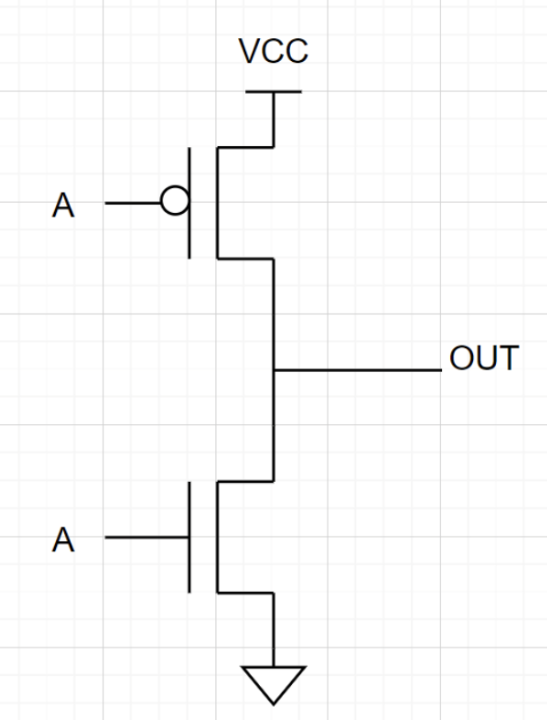
\includegraphics[width=0.5\textwidth]{figures/cmos1a_solution.png}
\end{figure}
\newpage

b. $ Z = (A \cdot B)'$
\begin{figure}[!h]
    \centering
    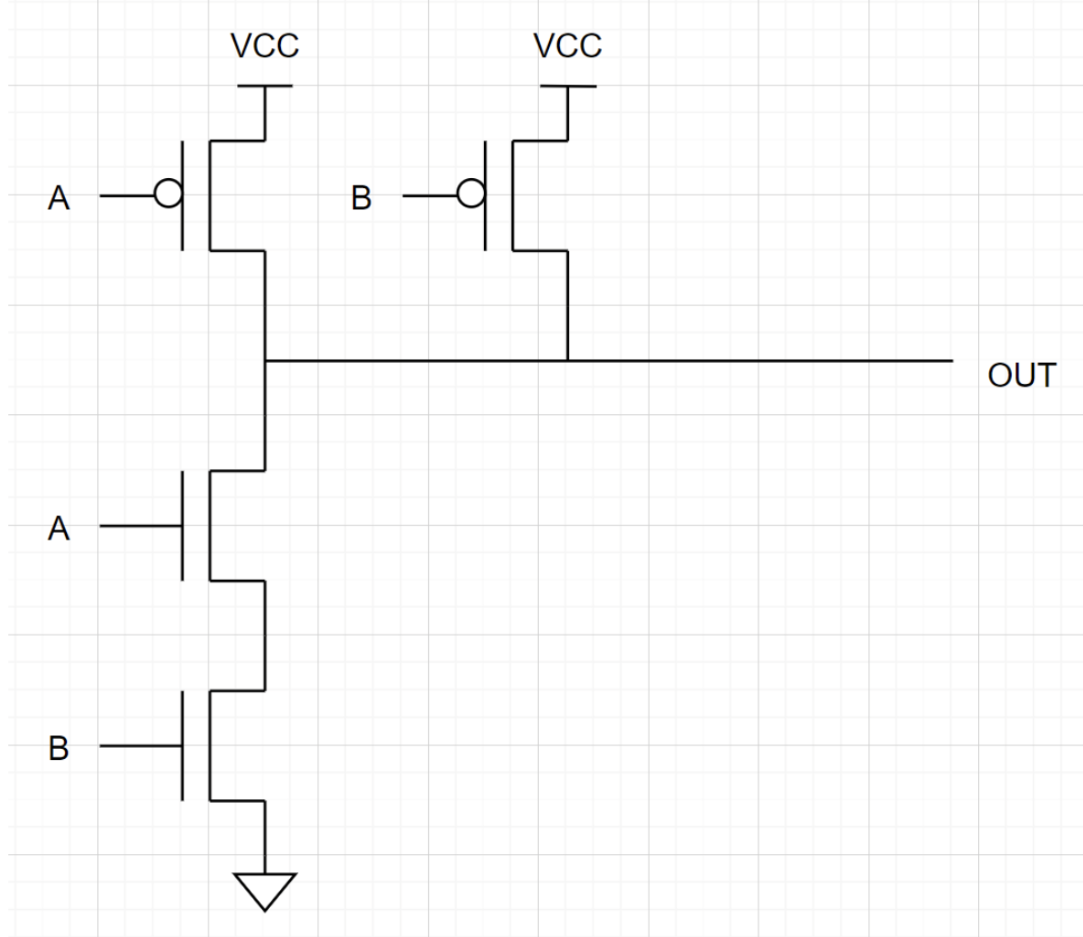
\includegraphics[width=0.8\textwidth]{figures/cmos1b_solution.png}
\end{figure}

c. $ Z = (A + B)'$
\begin{figure}[!h]
    \centering
    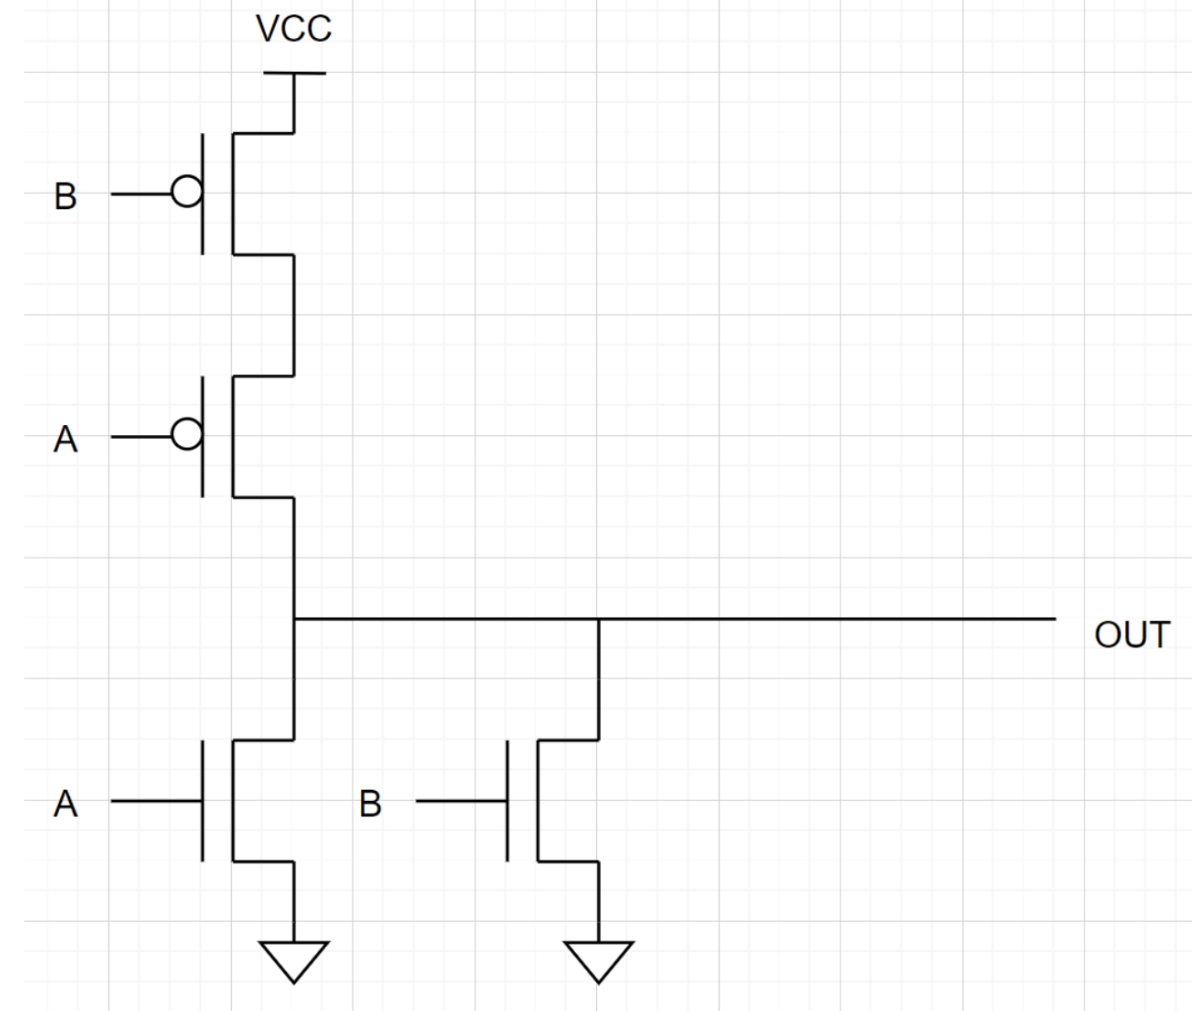
\includegraphics[width=0.8\textwidth]{figures/cmos1c_solution.png}
\end{figure}
\newpage
d. $ Z = ((A + B) \cdot C)'$
\begin{figure}[!h]
    \centering
    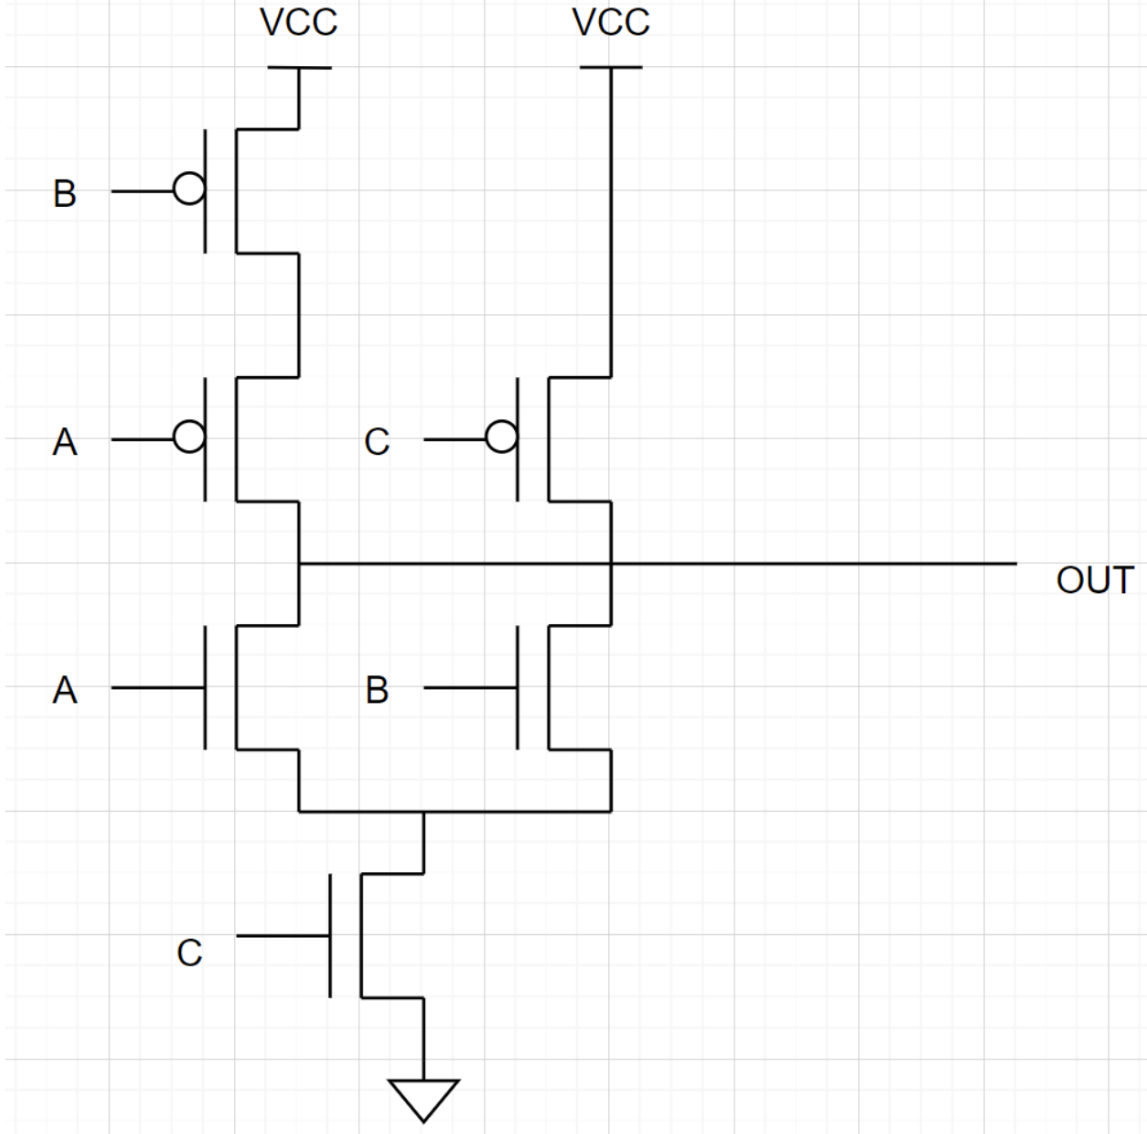
\includegraphics[width=0.7\textwidth]{figures/cmos1d_solution.png}
\end{figure}

e. $ Z = ((B \cdot C) + A)'$
\begin{figure}[!h]
    \centering
    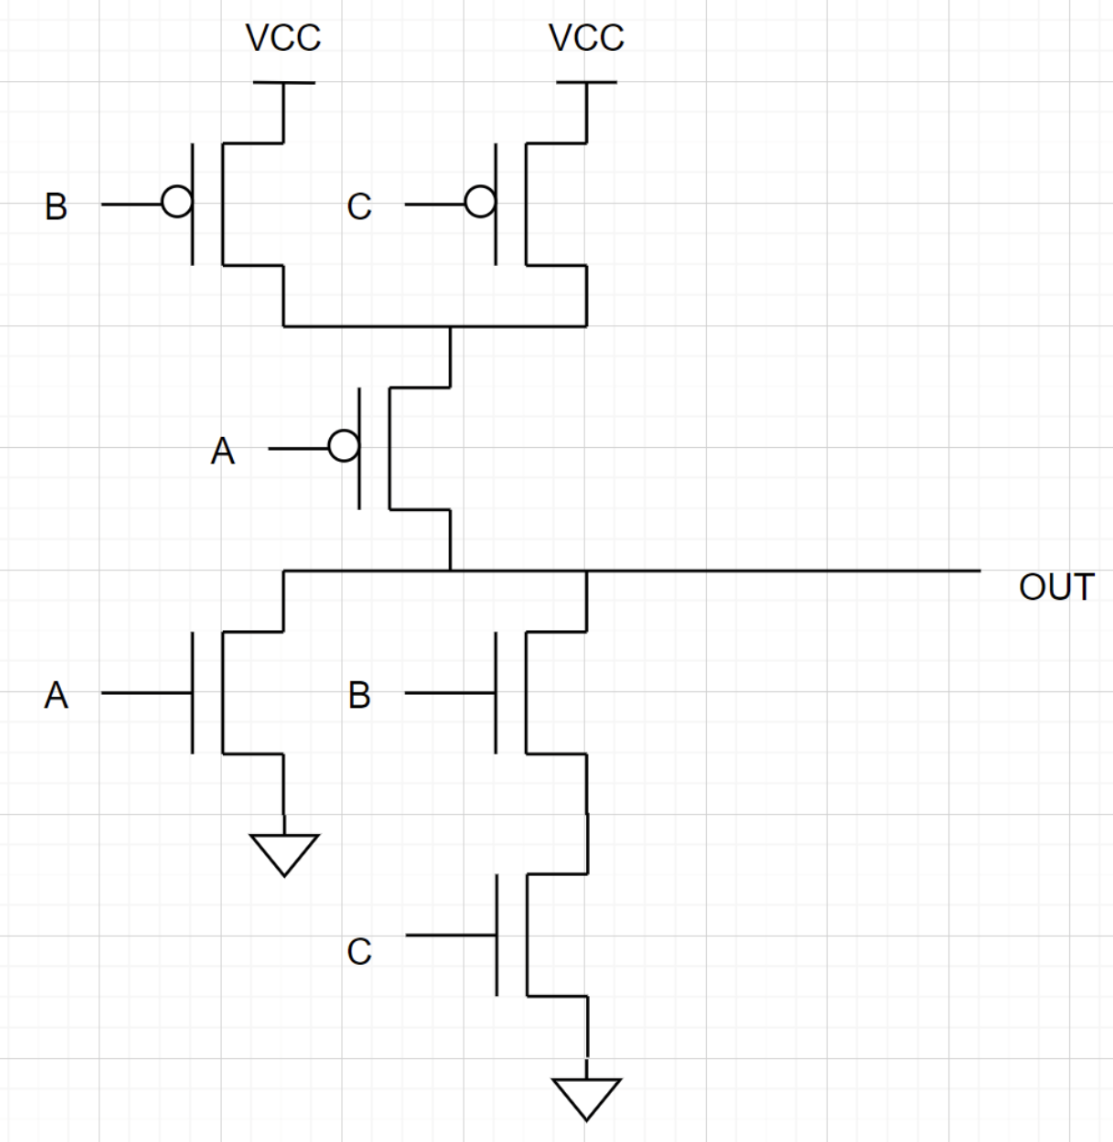
\includegraphics[width=0.7\textwidth]{figures/cmos1e_solution.png}
\end{figure}
\newpage
\subsection*{Problem 2}
Are these valid CMOS networks? If not, explain why. \\

a.
\begin{figure}[!h]
        \centering
        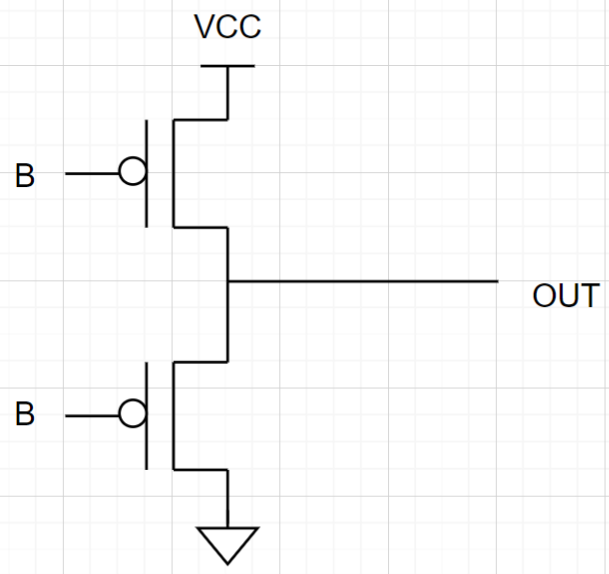
\includegraphics[width=0.6\textwidth]{figures/CMOS_2a.png}
\end{figure}
\\
\textbf{No. Notice that there is a P-type MOSFET used at the bottom. The output is not connected (left floating) when $B = 0$, and power is connected (shorted) to ground when $B = 1$.}

\newpage

b.
\begin{figure}[!h]
        \centering
        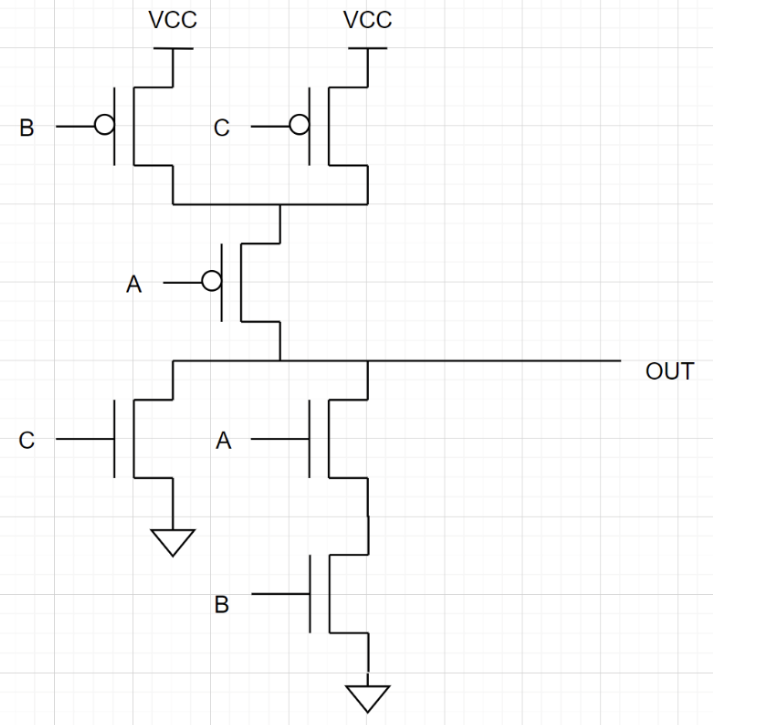
\includegraphics[width=0.9\textwidth]{figures/CMOS_2b.png}
\end{figure}
\\
\textbf{No, if $A = 0$, $B = 0$, $C = 1$, power is connected (shorted) to ground, and if $A = 1$, $B = 0$, $C = 0$, the output is left floating.}

\newpage
\section*{Boolean Expressions, Algebra, \& Optimization}
\subsection*{Problem 1}
Simplify the following expressions:
\begin{enumerate}[label=\alph*.]
    \item $ F(A,B,C) = (A + B) \cdot (B' + C) 
    \cdot (A + C)$ \\
\textbf{Consensus:} $F=(A+B)\cdot(B'+C)$ \\

    \item $ F(A,B,C) = A'BC + ABC + ABC' + AB'C$ \\
\textbf{Distributive:} $F=A'BC+A(BC+BC'+B'C)$ \\
\textbf{Distributive:} $F=A'BC+A(B(C+C')+B'C)$ \\
\textbf{Complementarity:} $F=A'BC+A(B+B'C)$ \\
\textbf{Distributive:} $F=A'BC+A(B+B')(B+C)$ \\
\textbf{Identity:} $F=A'BC+A(B+C)$ \\
\textbf{Distributive:} $F=A'BC+AB+AC$ \\
\textbf{Distributive:} $F=B(A'C+A)+AC$ \\
\textbf{Distributive:} $F=B(A'+A)(C+A)+AC$ \\
\textbf{Complementarity + Identity + Distributive:} $F=BC+BA+AC$ \\
    
    \item $ F(A,B,C) = A' \cdot (A + B) + (A + B) \cdot (A + B')$ \\
\textbf{Distributive:} $F=A'A+A'B+AA+AB'+AB+BB'$ \\
\textbf{Idempotence/Complementarity:} $F=A'B+A+AB'+AB$ \\
\textbf{Distributive:} $F=A\cdot(1+B) + B\cdot(A+A')$ \\
\textbf{Idempotence/Identity:} $F=A+B$ \\
\end{enumerate}

\subsection*{Problem 2}
True or False:
\begin{enumerate}[label=\alph*.]
    \item The delay for the following expression is 2.

    \begin{figure}[!h]
        \centering
        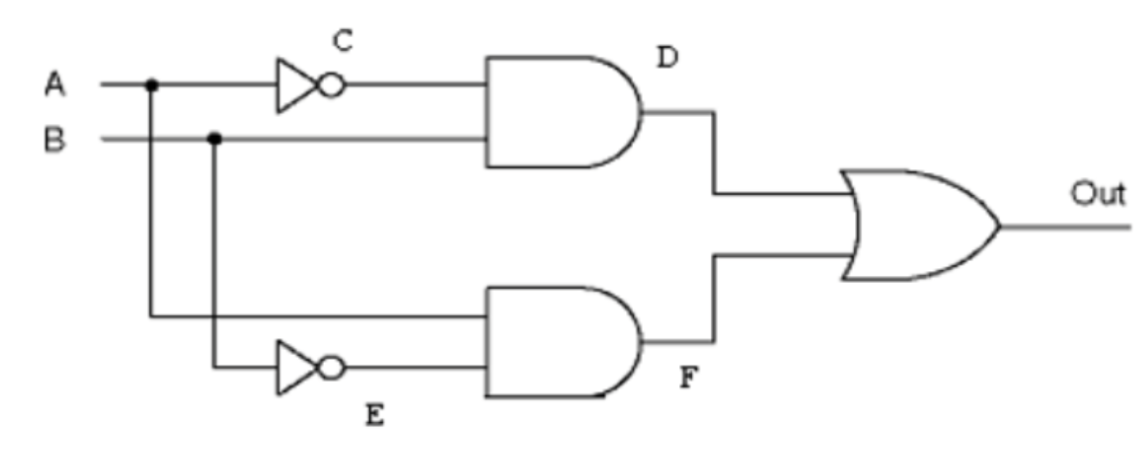
\includegraphics[width=0.7\textwidth]{figures/boolean2a.png}
    \end{figure}

\textbf{True. The maximum delay to get from an input to an output is through 2 gates, not including inverters. (we do not consider NOT gates as part of area or delay for ECE 120 area/delay heuristic)} 
    
    \item The area for the following expression is 7.

    \begin{figure}[!h]
        \centering
        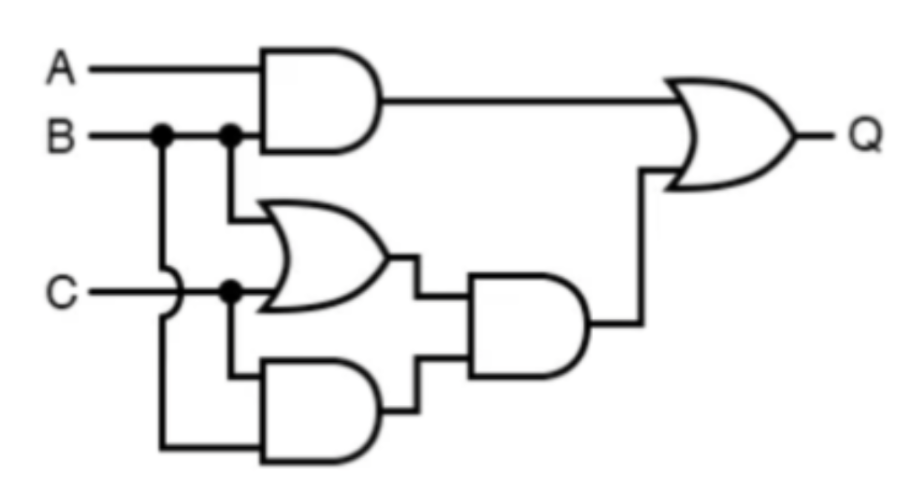
\includegraphics[width=0.7\textwidth]{figures/boolean2b.png}
    \end{figure}

\textbf{False. The area heuristic is calculated as the number of literals in the base expression plus the number of gates. There are 6 literals that feed directly into gates, and 5 gates in total, so the area is 11.}
    
\end{enumerate}

\newpage
\section*{K-maps, SOP \& POS Expressions}
\subsection*{Problem 1}
Use K-maps or simplification to find the minimal SOP and POS expressions for the following, then draw them in NAND/NOR form:\\

a. 
    \begin{table}[!h]
    \centering
\begin{tabular}{|c|c|c|c|}
\hline
\textbf{B} & \textbf{C} & \textbf{D} & \textbf{Z} \\ \hline 
0          & 0          & 0          & 1          \\ \hline 
0          & 0          & 1          & 0          \\ \hline 
0          & 1          & 0          & 1          \\ \hline 
0          & 1          & 1          & 1          \\ \hline 
1          & 0          & 0          & 0          \\ \hline 
1          & 0          & 1          & 0          \\ \hline 
1          & 1          & 0          & X          \\ \hline 
1          & 1          & 1          & 1          \\ \hline
\end{tabular}
\end{table} \\
\begin{figure}[!h]
\centering
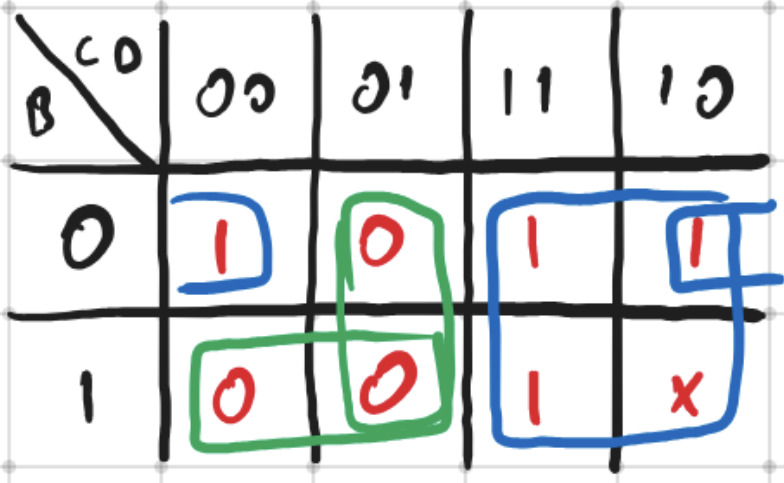
\includegraphics[width=0.4\textwidth]{figures/kmap1a_solution.png} \\
\caption*{\textbf{SOP: } $Z=C+B'D'$ \\
\textbf{POS: } $(B'+C)\cdot(C+D')$ \\}
\end{figure}
\newpage
b.
\begin{table}[!h]
\centering
\begin{tabular}{|l|l|l|l|l|}
\hline
\textbf{A} & \textbf{B} & \textbf{C} & \textbf{D} & \textbf{Z} \\ \hline
0          & 0          & 0          & 0          & 0          \\ \hline
0          & 0          & 0          & 1          & 1          \\ \hline
0          & 0          & 1          & 0          & 1          \\ \hline
0          & 0          & 1          & 1          & 1          \\ \hline
0          & 1          & 0          & 0          & 0          \\ \hline
0          & 1          & 0          & 1          & 0          \\ \hline
0          & 1          & 1          & 0          & X          \\ \hline
0          & 1          & 1          & 1          & X          \\ \hline
1          & 0          & 0          & 0          & 0          \\ \hline
1          & 0          & 0          & 1          & 1          \\ \hline
1          & 0          & 1          & 0          & 0          \\ \hline
1          & 0          & 1          & 1          & 0          \\ \hline
1          & 1          & 0          & 0          & 0          \\ \hline
1          & 1          & 0          & 1          & X          \\ \hline
1          & 1          & 1          & 0          & X          \\ \hline
1          & 1          & 1          & 1          & X          \\ \hline
\end{tabular}
\end{table}

\begin{figure}[!h]
\centering
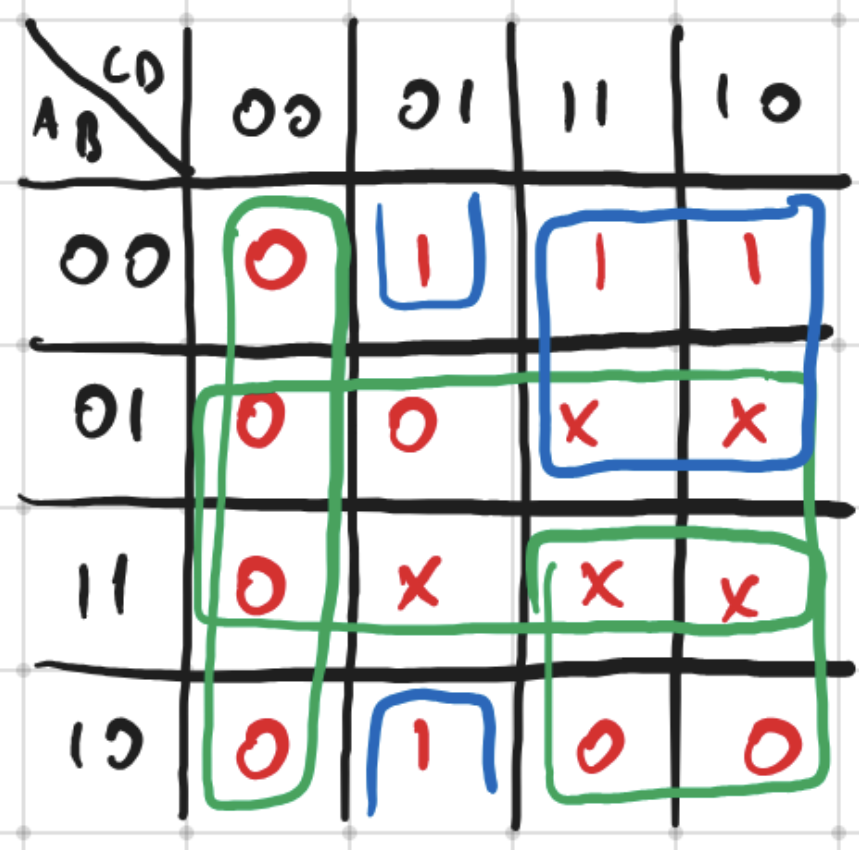
\includegraphics[width=0.4\textwidth]{figures/kmap1b_solution.png} \\
\textbf{SOP: } $Z=A'C+B'C'D$ \\
\textbf{POS: } $B' \cdot (C+D) \cdot (A'+C')$ \\
\end{figure}
\newpage

\section*{Adders, ALUs, and Bit-Slicing}
\subsection*{Problem 1}
Remember that the logical output for one slice of a full adder is:
\begin{table}[!h]
\centering
\begin{tabular}{|l|l|l|l|l|}
\hline
\textbf{A} & \textbf{B} & \textbf{Cin} & \textbf{Cout} & \textbf{S} \\ \hline
0          & 0          & 0            & 0             & 0          \\ \hline
0          & 0          & 1            & 0             & 1          \\ \hline
0          & 1          & 0            & 0             & 1          \\ \hline
0          & 1          & 1            & 1             & 0          \\ \hline
1          & 0          & 0            & 0             & 1          \\ \hline
1          & 0          & 1            & 1             & 0          \\ \hline
1          & 1          & 0            & 1             & 0          \\ \hline
1          & 1          & 1            & 1             & 1          \\ \hline
\end{tabular}
\end{table}

\begin{enumerate}[label=\alph*.]
    \item Find an expression for Cout and S using AND and OR gates.\\
    \textbf{Multiple possible solutions. Use K-maps or simplify the boolean expressions.}\\
    $S = A \bigoplus B \bigoplus Cin$ \\
    $S = (AB' + A'B) \bigoplus Cin$ \\
    $S = (AB')' \cdot Cin + (AB') \cdot Cin' + (A'B)' \cdot Cin + (A'B) \cdot Cin'$ \\
    \\
    $Cout = AB + AC + BC$
    
    \item Consider the digital circuit: 
    \begin{figure}[!h]
        \centering
        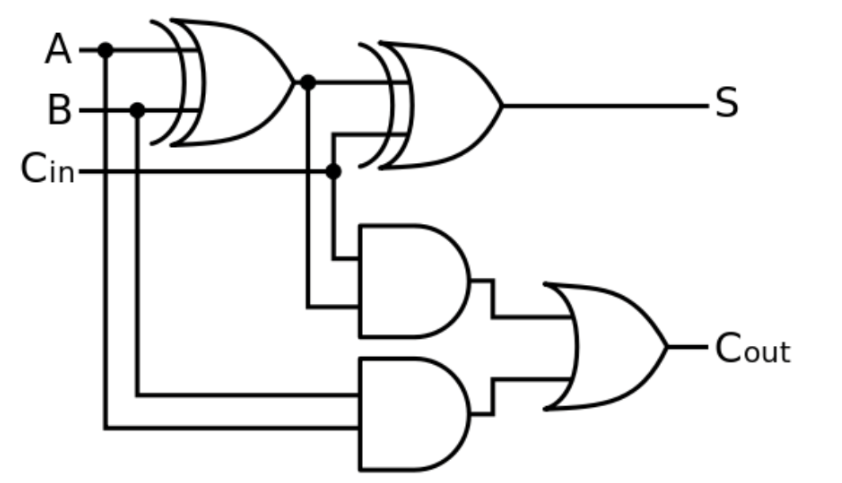
\includegraphics[width=0.7\textwidth]{figures/adder1b.png}
    \end{figure}
    \\ Verify that it is equivalent to your expression. \\
    \textbf{Trace out the inputs from the truth table, you should get the same results for S.}
\end{enumerate}

\subsection*{Problem 2}
Build each of these circuits using only adders, inverters, and fixed inputs (1 or 0). Do not account for overflows unless otherwise noted.
\begin{enumerate}[label=\alph*.]
    \item For two 4-bit unsigned integers $A_3A_2A_1A_0$ and $B_3B_2B_1B_0$, calculate the 5-bit unsigned integer $S_4S_3S_2S_1S_0 = A + B$. \\
    \begin{figure}[!h]
        \centering
        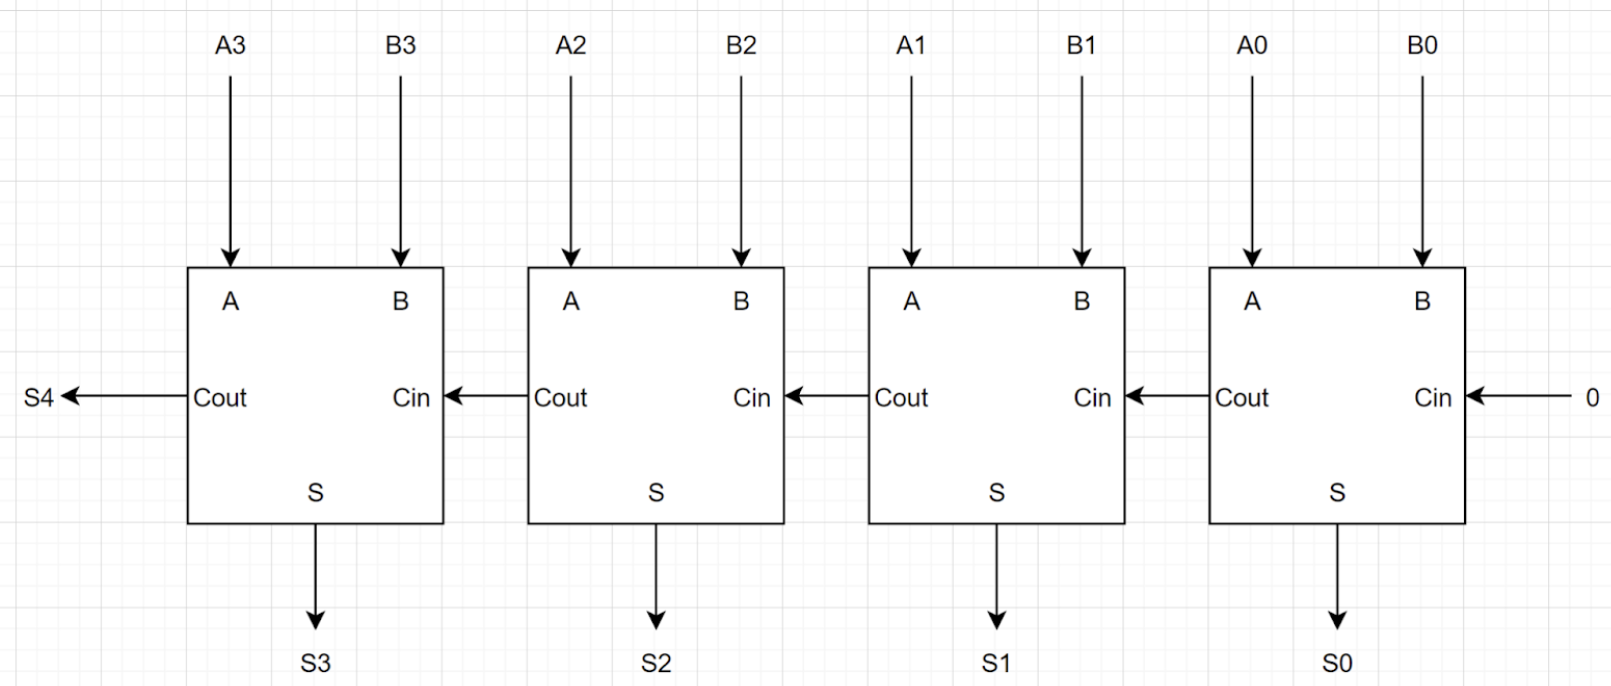
\includegraphics[width=1\textwidth]{figures/adder2a_solution.png}
    \end{figure}
    
    \item For two 4-bit two's complement integers $A_3A_2A_1A_0$ and $B_3B_2B_1B_0$ , calculate the 4-bit two's complement integer $S_3S_2S_1A_0$ where $S=A-B$. \\
    \begin{figure}[!h]
        \centering
        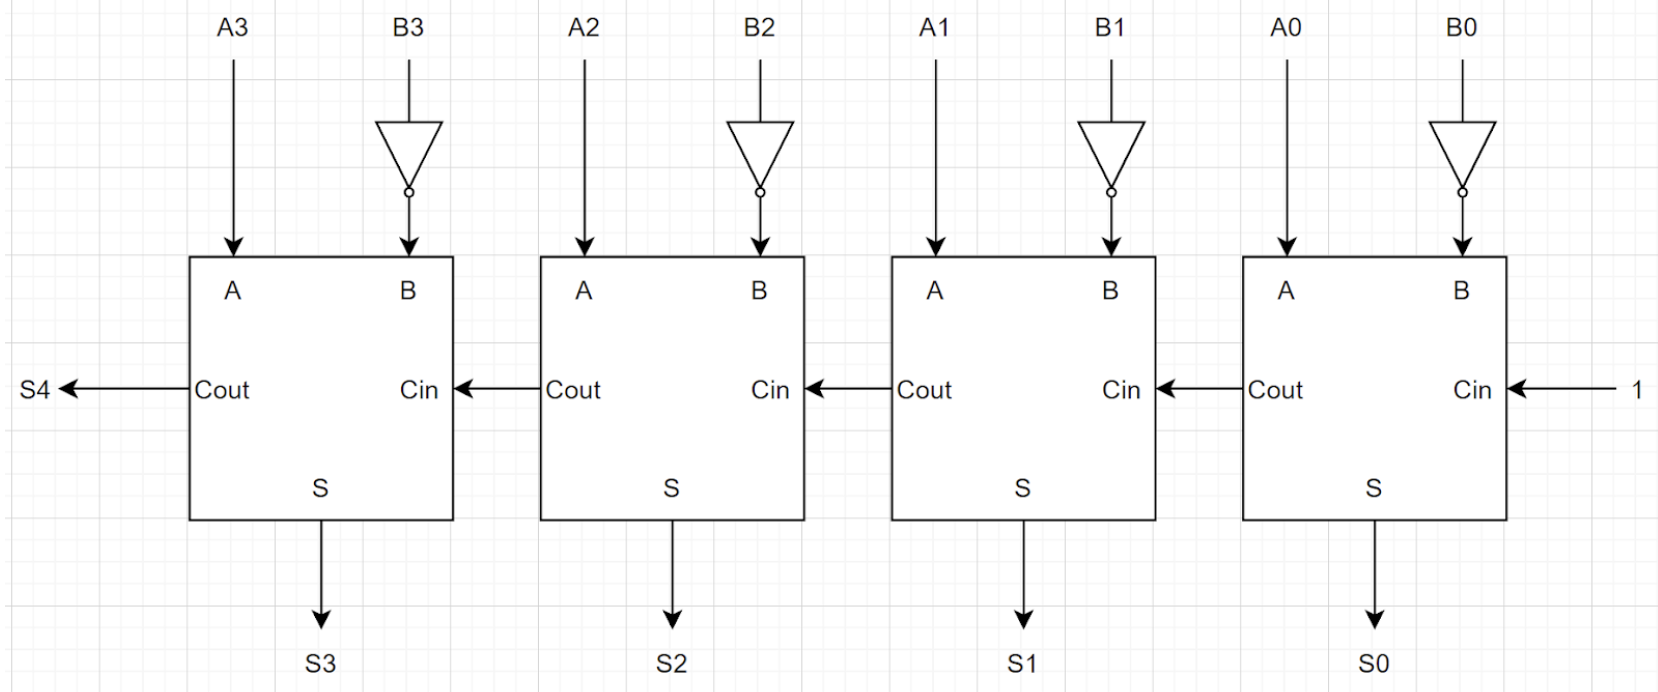
\includegraphics[width=1\textwidth]{figures/adder2b_solution.png}
    \end{figure}
    \newpage
    \item For three 3-bit two's complement integers $A_2A_1A_0$, $B_2B_1B_0$, $C_2C_1C_0$, calculate $S_2S_1S_0=A+A-B-C$. \\
    $S_2S_1S_0 = (A-B)+(A-C)$\\
    \begin{figure}[!h]
        \centering
        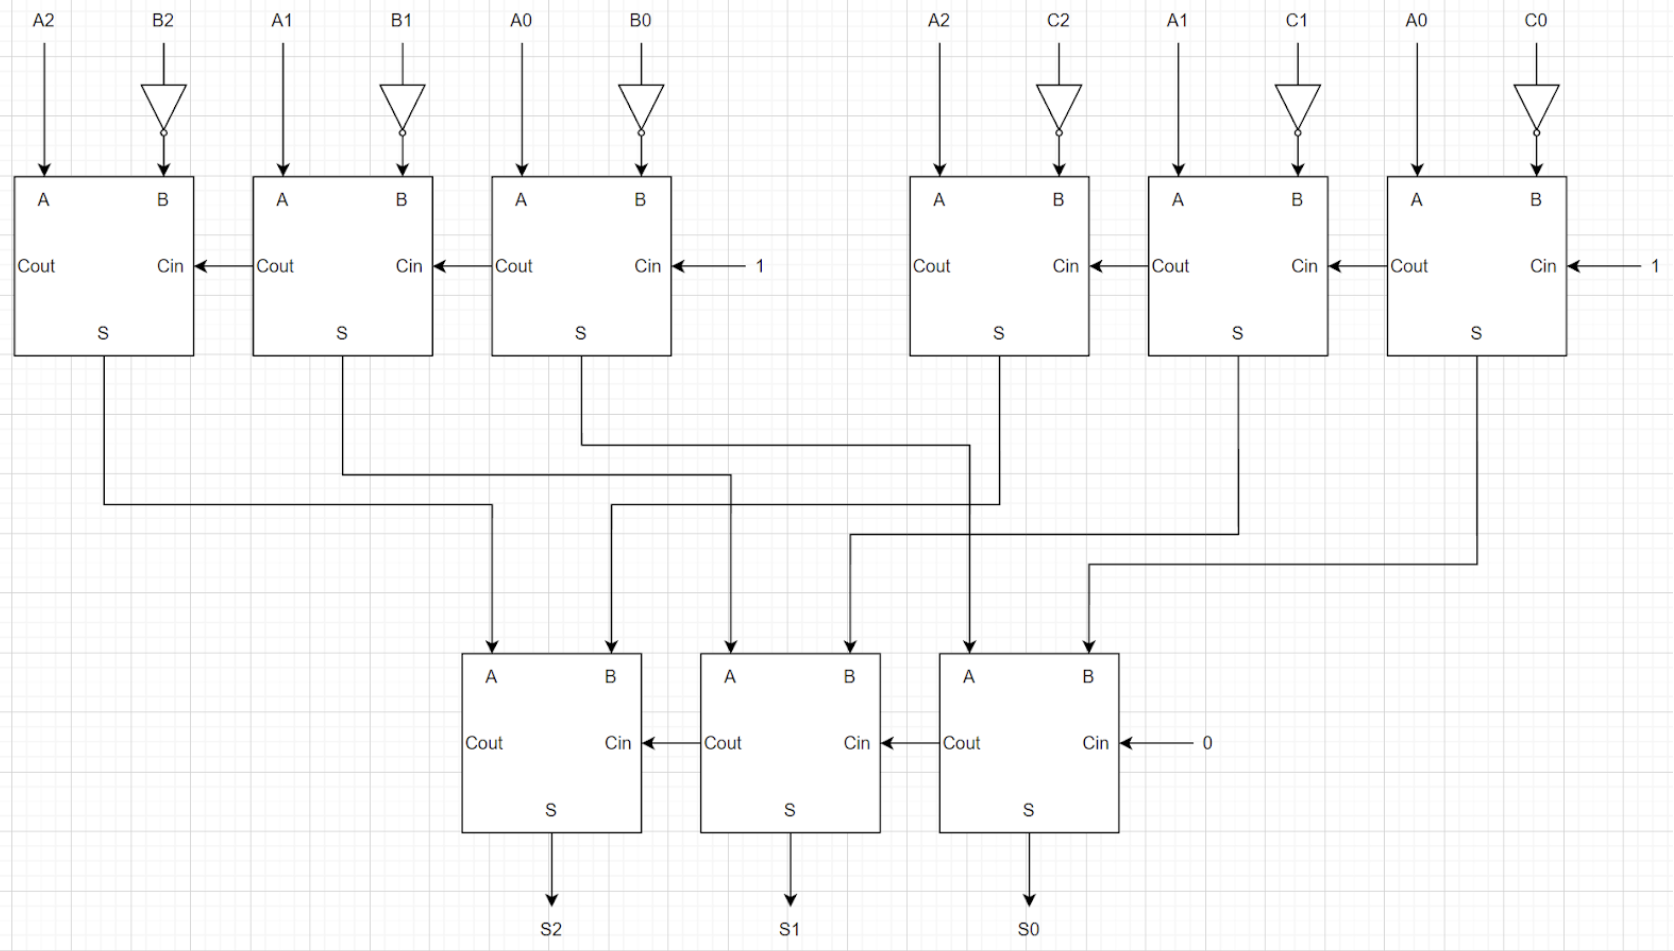
\includegraphics[width=1\textwidth]{figures/adder2c_solution.png}
    \end{figure}
\end{enumerate}

\newpage
\subsection*{Problem 3}
Assume an ALU that takes two 8-bit integers $A$ and $B$ as input and can calculate $AB$ (AND), 
\begin{enumerate}[label=\alph*.]
    \item How many bits is the output $S$? \\
    \textbf{8 bits.}
    \item How many bits must the control signal be? \\
    \textbf{At least 2 bits. There are 3 operations, which is less than $2^2$.}
    \item Is the ALU logically complete? Assume you have 0 and 1 available. \\
    \textbf{(multiple possible ways to show this)
We know that the set {AND, OR, NOT} is logically complete (Lumetta 1.4.5), so we want to show that we can produce these operations using the operations we are given.
We already have AND, so we want to make OR and NOT.
For NOT, we know that any $A\bigoplus1=A'$, and we are given logical 1.
For OR, one way to do this is by adding $(A\bigoplus B)+(AB)$.}
\begin{table}[!h]
\centering
\begin{tabular}{|l|l|l|l|l|}
\hline
A & B & $A\bigoplus B$ & $AB$ & $(A\bigoplus B)+(AB)$ \\ \hline
0 & 0 & 0  & 0  & 0         \\ \hline
0 & 1 & 1  & 0  & 1         \\ \hline
1 & 0 & 1  & 0  & 1         \\ \hline
1 & 1 & 0  & 1  & 1         \\ \hline
\end{tabular}
\end{table}\\
\textbf{
We can see by the truth table that this is equivalent to OR.
		We also don’t have to worry about the carry as at most one of its inputs are 1.
		Thus, the set {AND, XOR, ADD} is logically complete.
}

    \item (Optional) Draw out the full circuit diagram for this ALU, using basic logic gates, MUXs, decoders, and full adders.
\end{enumerate}


\subsection*{Problem 4}
In 50 or fewer words, explain the advantages and disadvantages of bit-slicing over optimizing for many variables.\\
\textbf{Bit-slicing allows for per-bit design, which may be simpler to implement, and usually results in much smaller area in exchange for a larger delay. 
Optimizing for many variables can yield results in as little as a delay of 2 (two-level logic), but uses many more gates and much larger area.}

\newpage
\section*{Multiplexers}
\subsection*{Problem 1}
Write down the truth table for a 2-to-1 multiplexer. Write an expression for the output, and implement the 2:1 MUX using AND gates, OR gates, and inverters.

\begin{table}[!h]
\centering
\begin{tabular}{|l|l|l|l|}
\hline
\textbf{I0} & \textbf{I1} & \textbf{S} & \textbf{Y} \\ \hline
0           & 0           & 0          & 0          \\ \hline
0           & 0           & 1          & 0          \\ \hline
0           & 1           & 0          & 0          \\ \hline
0           & 1           & 1          & 1          \\ \hline
1           & 0           & 0          & 1          \\ \hline
1           & 0           & 1          & 0          \\ \hline
1           & 1           & 0          & 1          \\ \hline
1           & 1           & 1          & 1          \\ \hline
\end{tabular}
\end{table}
$$\mathbf{Y=(I_0S'+I_1S)}$$
\begin{figure}[!h]
    \centering
    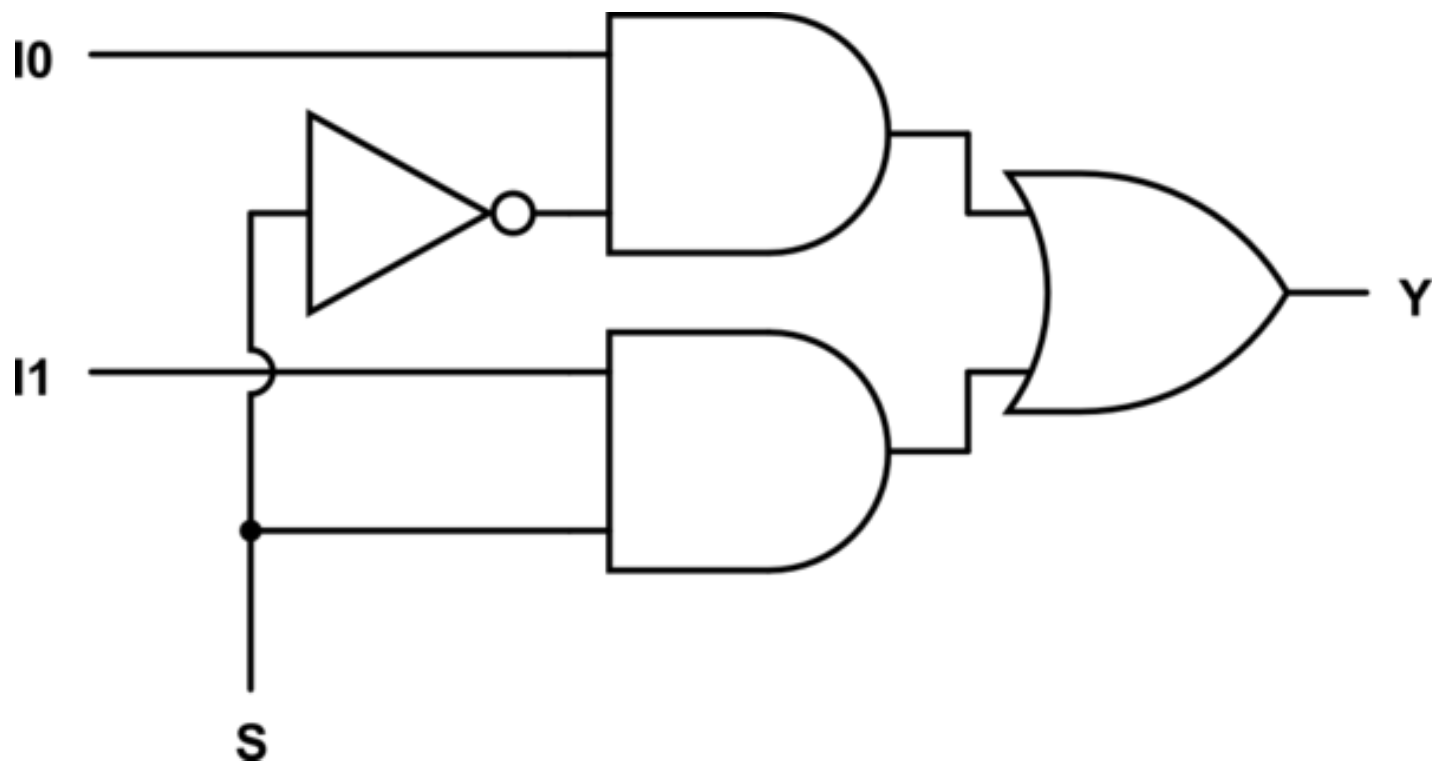
\includegraphics[width=0.6\textwidth]{figures/mux1_solution.png}
\end{figure}

\newpage
\subsection*{Problem 2}
Using the same process (you may not need the truth table), implement a 4:1 MUX using AND gates, OR gates, and inverters.
\begin{figure}[!h]
    \centering
    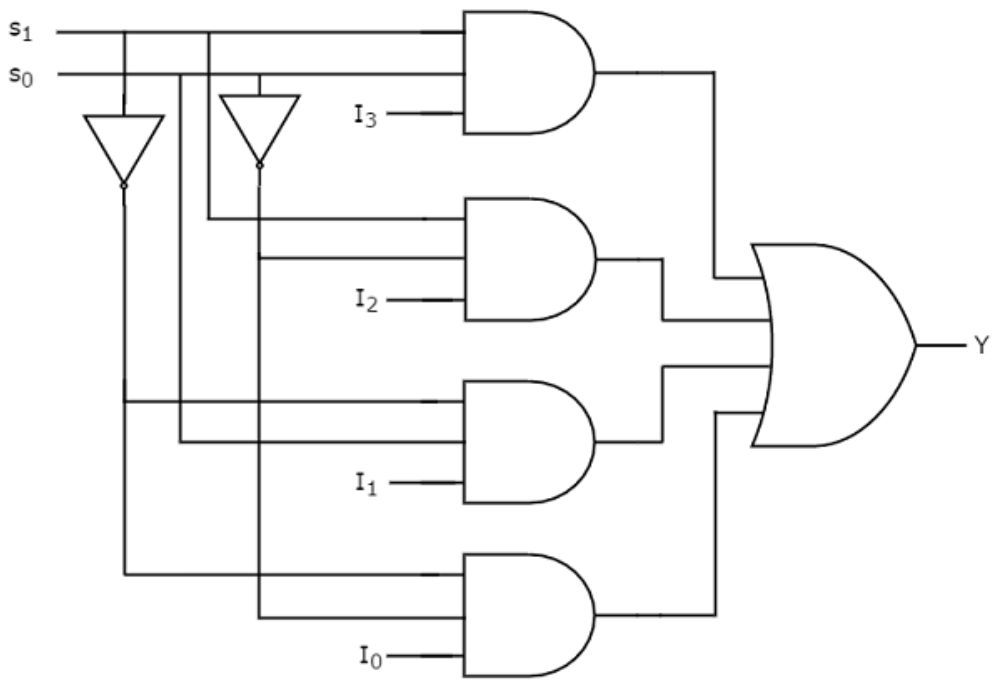
\includegraphics[width=0.6\textwidth]{figures/mux2_solution.png}
\end{figure}


\subsection*{Problem 3}
Implement a 4:1 MUX using three 2:1 MUXs.
\begin{figure}[!h]
    \centering
    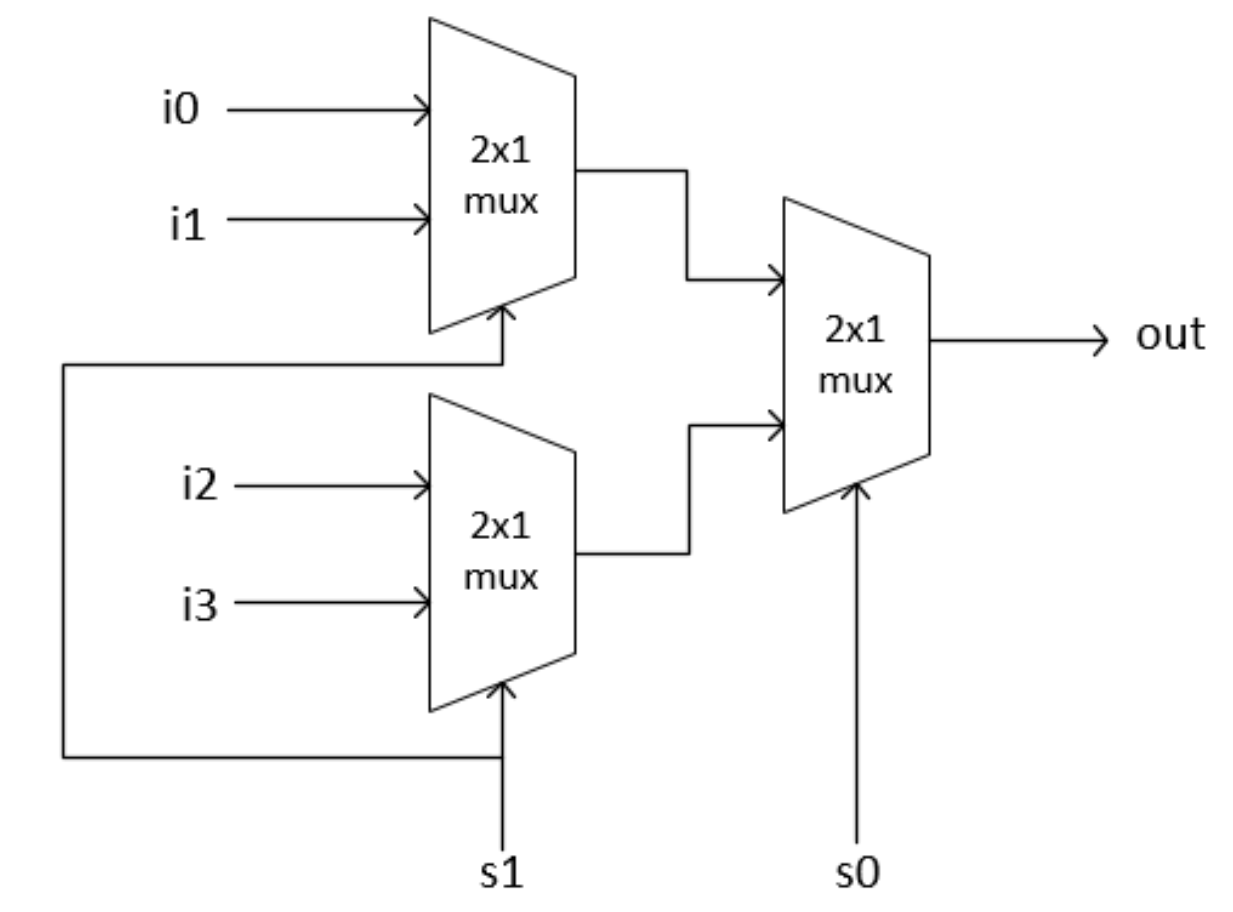
\includegraphics[width=0.6\textwidth]{figures/mux3_solution.png}
\end{figure}

\newpage
\subsection*{Problem 4}
Implement a 8:1 MUX using two 4:1 MUXs and a 2:1 MUX.
\begin{figure}[!h]
    \centering
    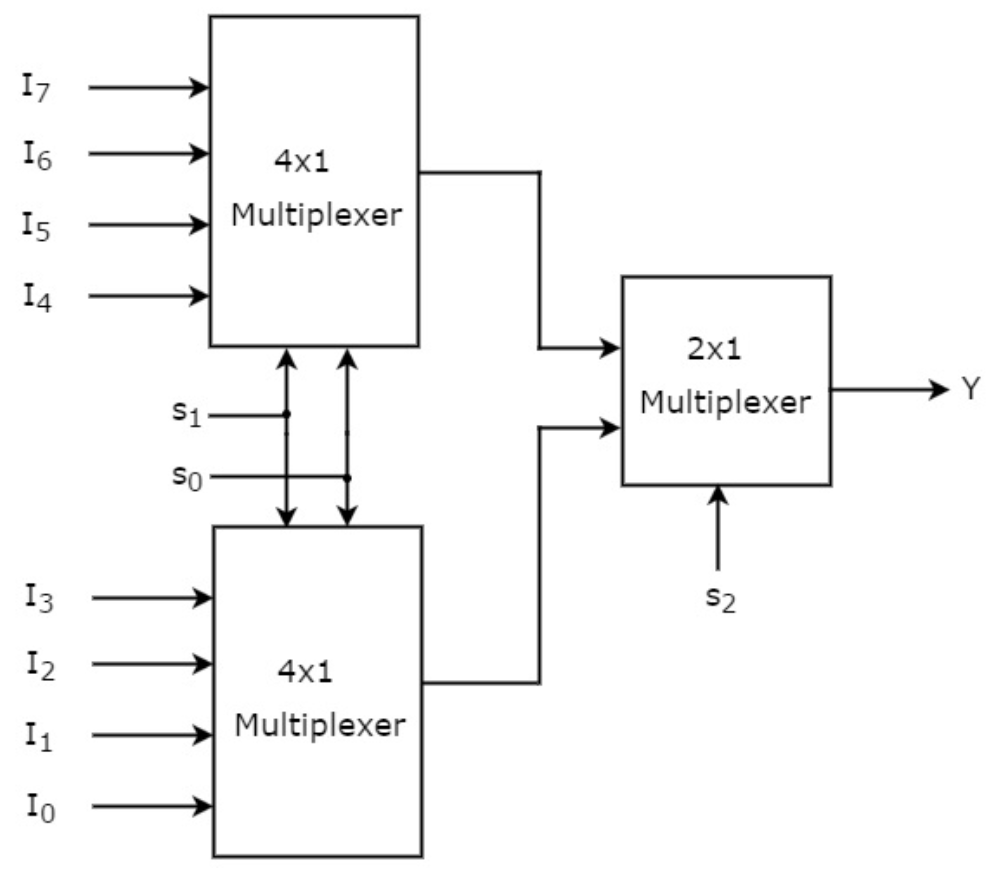
\includegraphics[width=0.6\textwidth]{figures/mux4_solution.png}
\end{figure}

\newpage
\section*{Decoders}
\subsection*{Problem 1}
In 20 words or less, what does a decoder do?\\
\textbf{Take an $N$-bit integer $I$ and output $1$ on $D_i$ and $0$ on all other $2^N-1$ outputs.}

\subsection*{Problem 2}
Implement a 2x4 decoder using AND gates, OR gates, and inverters.
\begin{figure}[!h]
    \centering
    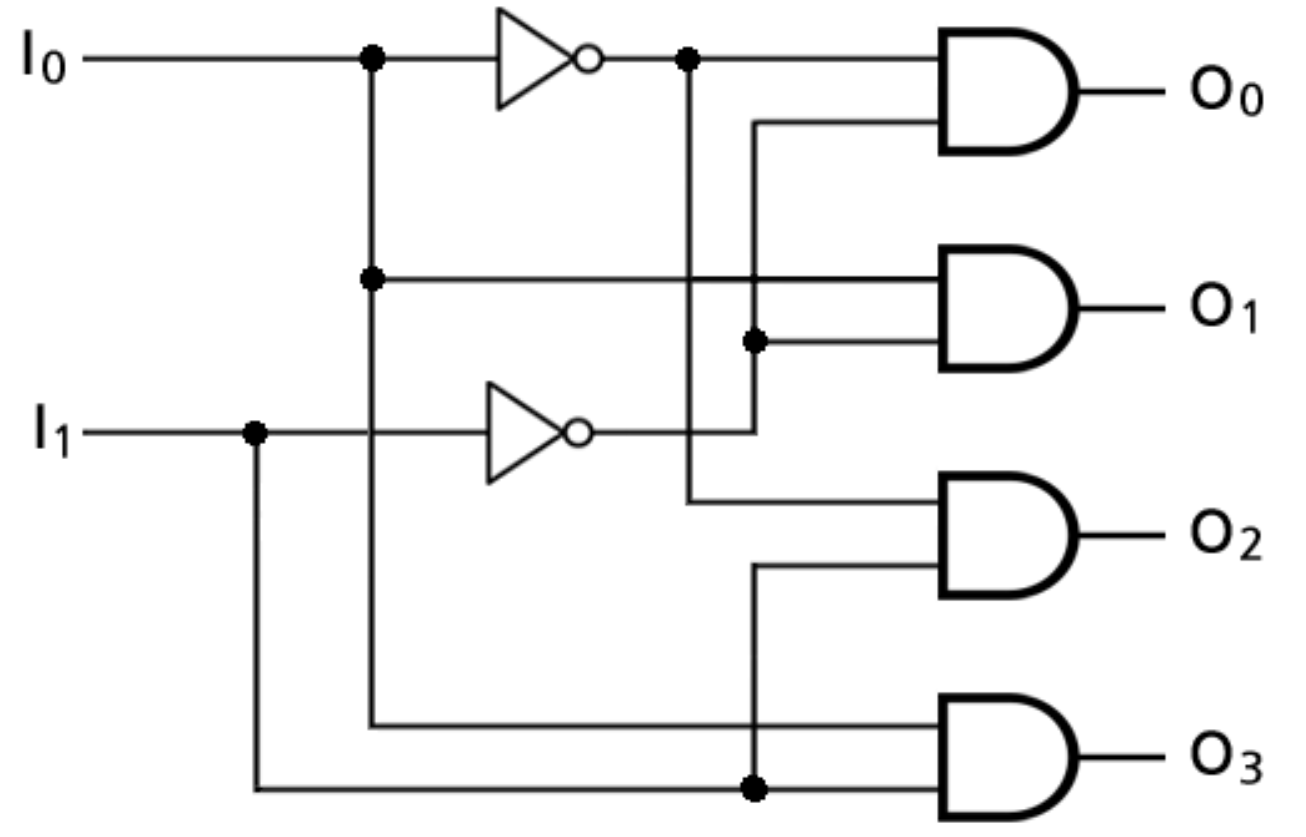
\includegraphics[width=0.6\textwidth]{figures/decoder2_solution.png}
\end{figure}
\newpage
\subsection*{Problem 3}
Implement a 4x16 decoder using five 2x4 decoders. (Hint: you should use the ENABLE pin)
\begin{figure}[!h]
    \centering
    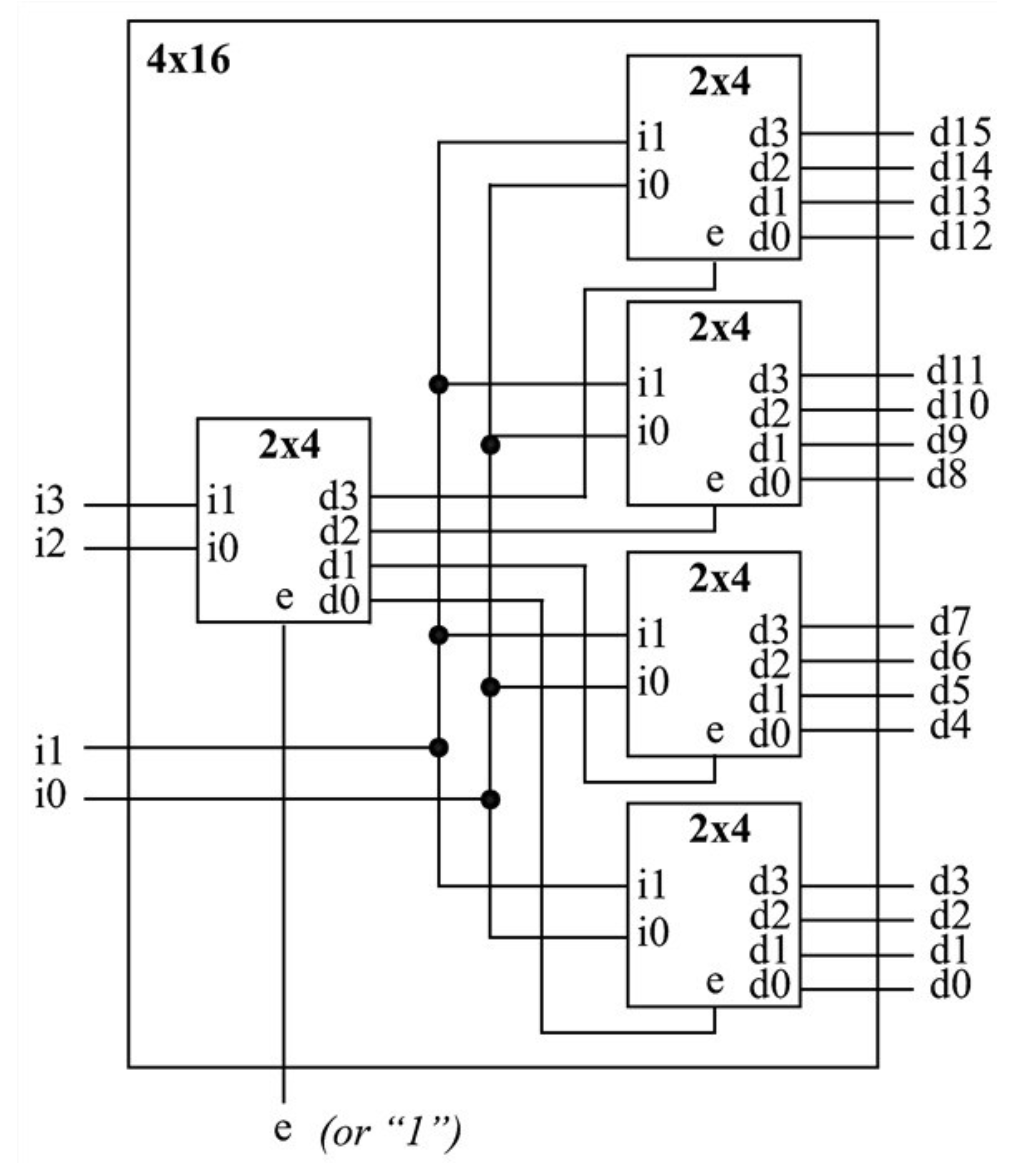
\includegraphics[width=0.6\textwidth]{figures/decoder3_solution.png}
\end{figure}
\\ \textbf{Note: you can also do this without the ENABLE pin by adding an AND gate for every output.}

\newpage
\section*{Latches \& Flip-Flops}
\subsection*{Problem 1}
Find the stable states of the following latches: \\

a.
    \begin{figure}[!h]
        \centering
        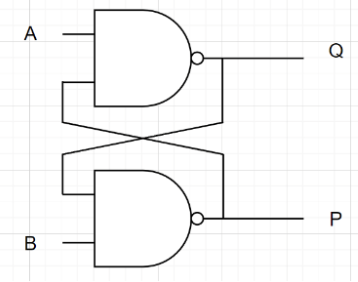
\includegraphics[width=0.7\textwidth]{figures/latch1a.png}
    \end{figure}

    \begin{table}[!h]
    \centering
\begin{tabular}{|c|c|c|c|}
\hline
\textbf{A} & \textbf{B} & \textbf{Q} & \textbf{P} \\ \hline
0          & 0          & 1          & 1          \\ \hline
0          & 1          & 1          & 0          \\ \hline
1          & 0          & 0          & 1          \\ \hline
1          & 1          & 0          & 1          \\ \hline
1          & 1          & 1          & 0          \\ \hline
\end{tabular}
\end{table}

\newpage
b.
    \begin{figure}[!h]
        \centering
        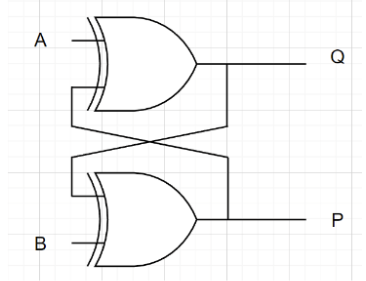
\includegraphics[width=0.5\textwidth]{figures/latch1b.png}
    \end{figure}

    \begin{table}[!h]
    \centering
\begin{tabular}{|c|c|c|c|}
\hline
\textbf{A} & \textbf{B} & \textbf{Q} & \textbf{P} \\ \hline
0          & 0          & 0          & 0          \\ \hline
0          & 0          & 1          & 1          \\ \hline
1          & 1          & 1          & 0          \\ \hline
1          & 1          & 0          & 1          \\ \hline
\end{tabular}
\end{table}

c. Which latch is more viable for data storage? \\
\textbf{Try to store some data on the XOR latch: \href{https://www.falstad.com/circuit/circuitjs.html?ctz=CQAgjCAMB0l3BWcMBMcUHYMGZIA4UA2ATmIxAUgoqoQFMBaMMAKAHcQUFDP8RtCeXkMjtO3fpAAs-QZJmiAsrKFohUuMKidoCFsoFDcMjVWPaUulgBlwKIWGIoQeKo+duQAMwCGAGwBnOmpRWzB7fjQXMyjPX0DgpFEwBBlw1T4uHjULbT0UtIjzLPlcpD0OEpz0zjwRMRLzGpQUBRYgA}{Falstad Simulation} (click the inputs)\\
When we want to store data, we can only toggle one input at a time. (it’s impossible to synchronize two inputs changing at exactly the same time)\\
When we enter any unstable state, since the circuit flickers, it’s impossible to predict what Q and P end up storing. Thus, it’s not actually able to reliably store anything. 
Thus, the NAND latch is more viable.
}
\subsection*{Problem 2}
Explain the process of storing a bit of data in a D latch.
\begin{figure}[!h]
    \centering
    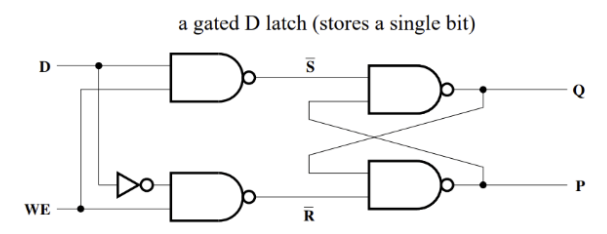
\includegraphics[width=0.5\textwidth]{figures/latch2.png}
\end{figure}\\

\textbf{When we want to store data, we set WE (write-enable) to high, which allows the two NAND gates on the left to toggle. Then, we toggle D, and Q mirrors the signal on D. Then to stop writing, we set WE to low.}

\subsection*{Problem 3}
Explain the difference between a D latch and a D flip-flop.
\\ \textbf{The output of a D latch updates as long as the WE (write-enable) signal is high. On the other hand, the output of a D flip flop only updates upon the rising/falling edge of the clock. (rising edge for a positive-edge triggered D flip flop and falling edge for a negative-edge triggered D flip flop).}

\subsection*{Problem 4}
Implement a 4-bit register using D flip-flops
\begin{figure}[!h]
    \centering
    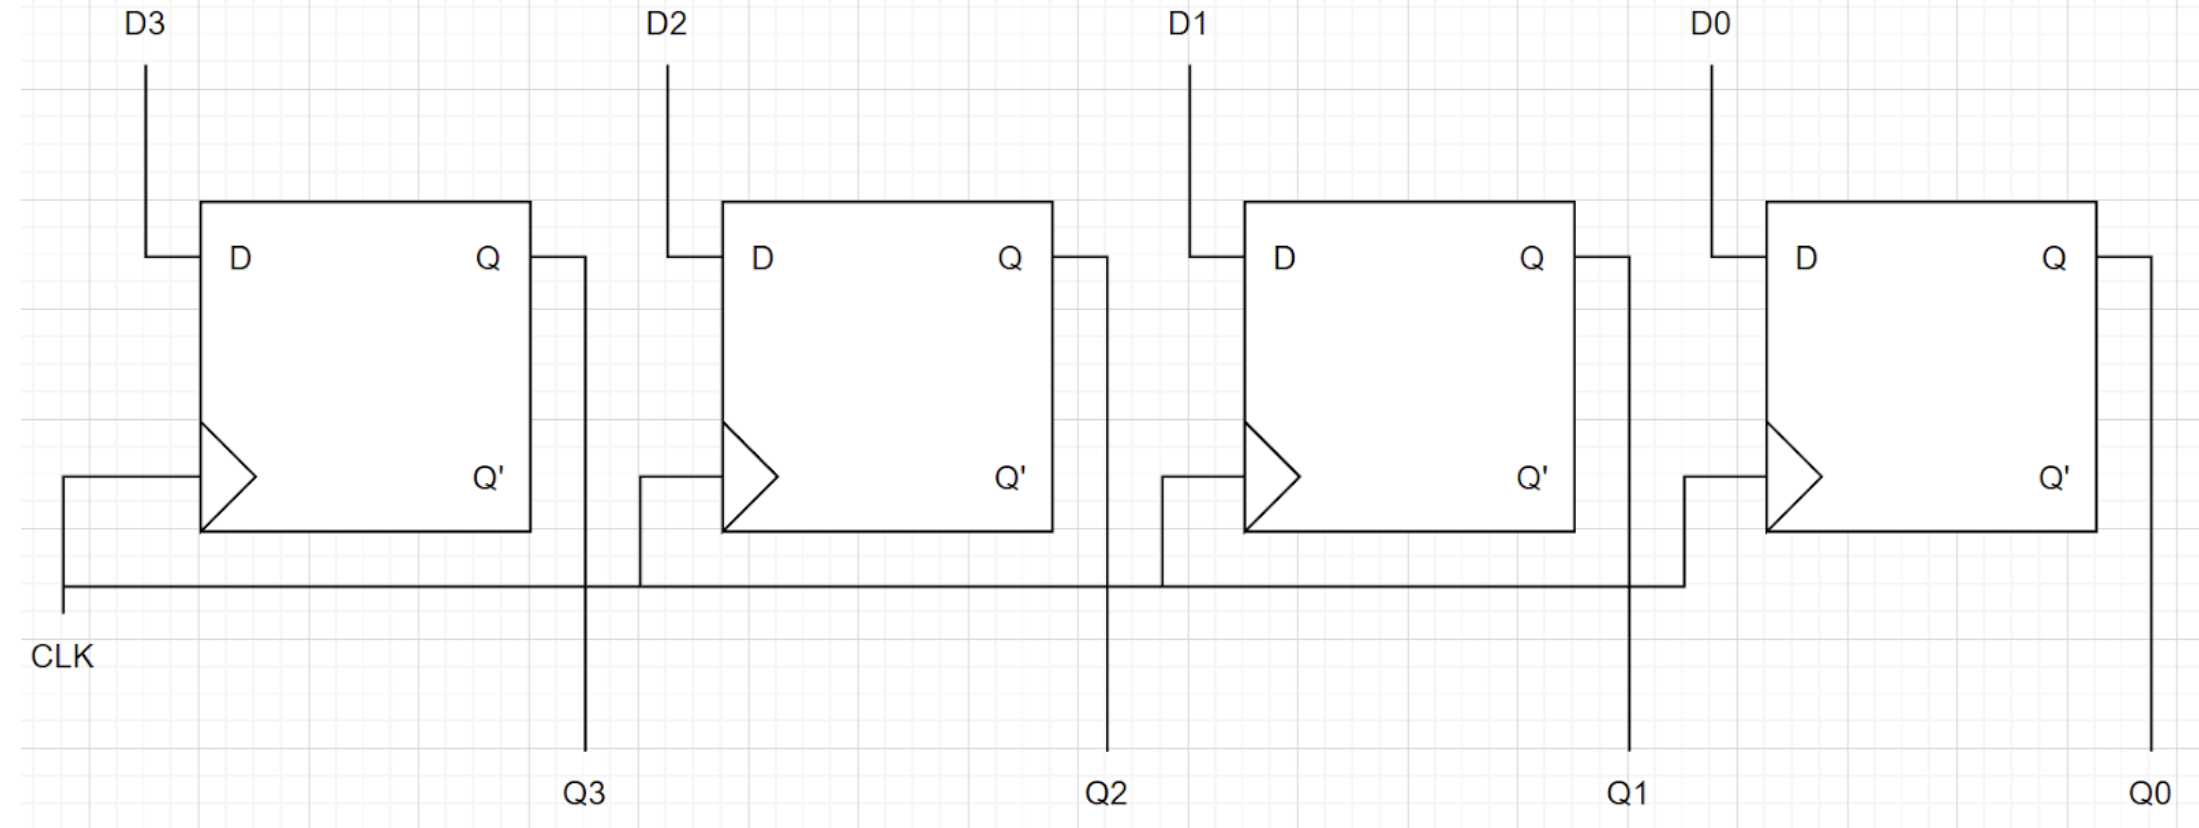
\includegraphics[width=0.9\textwidth]{figures/latch4_solution.png}
\end{figure}

\subsection*{Problem 5}
Implement a 4-bit shift register with MSB load using D flip-flops.
\begin{figure}[!h]
    \centering
    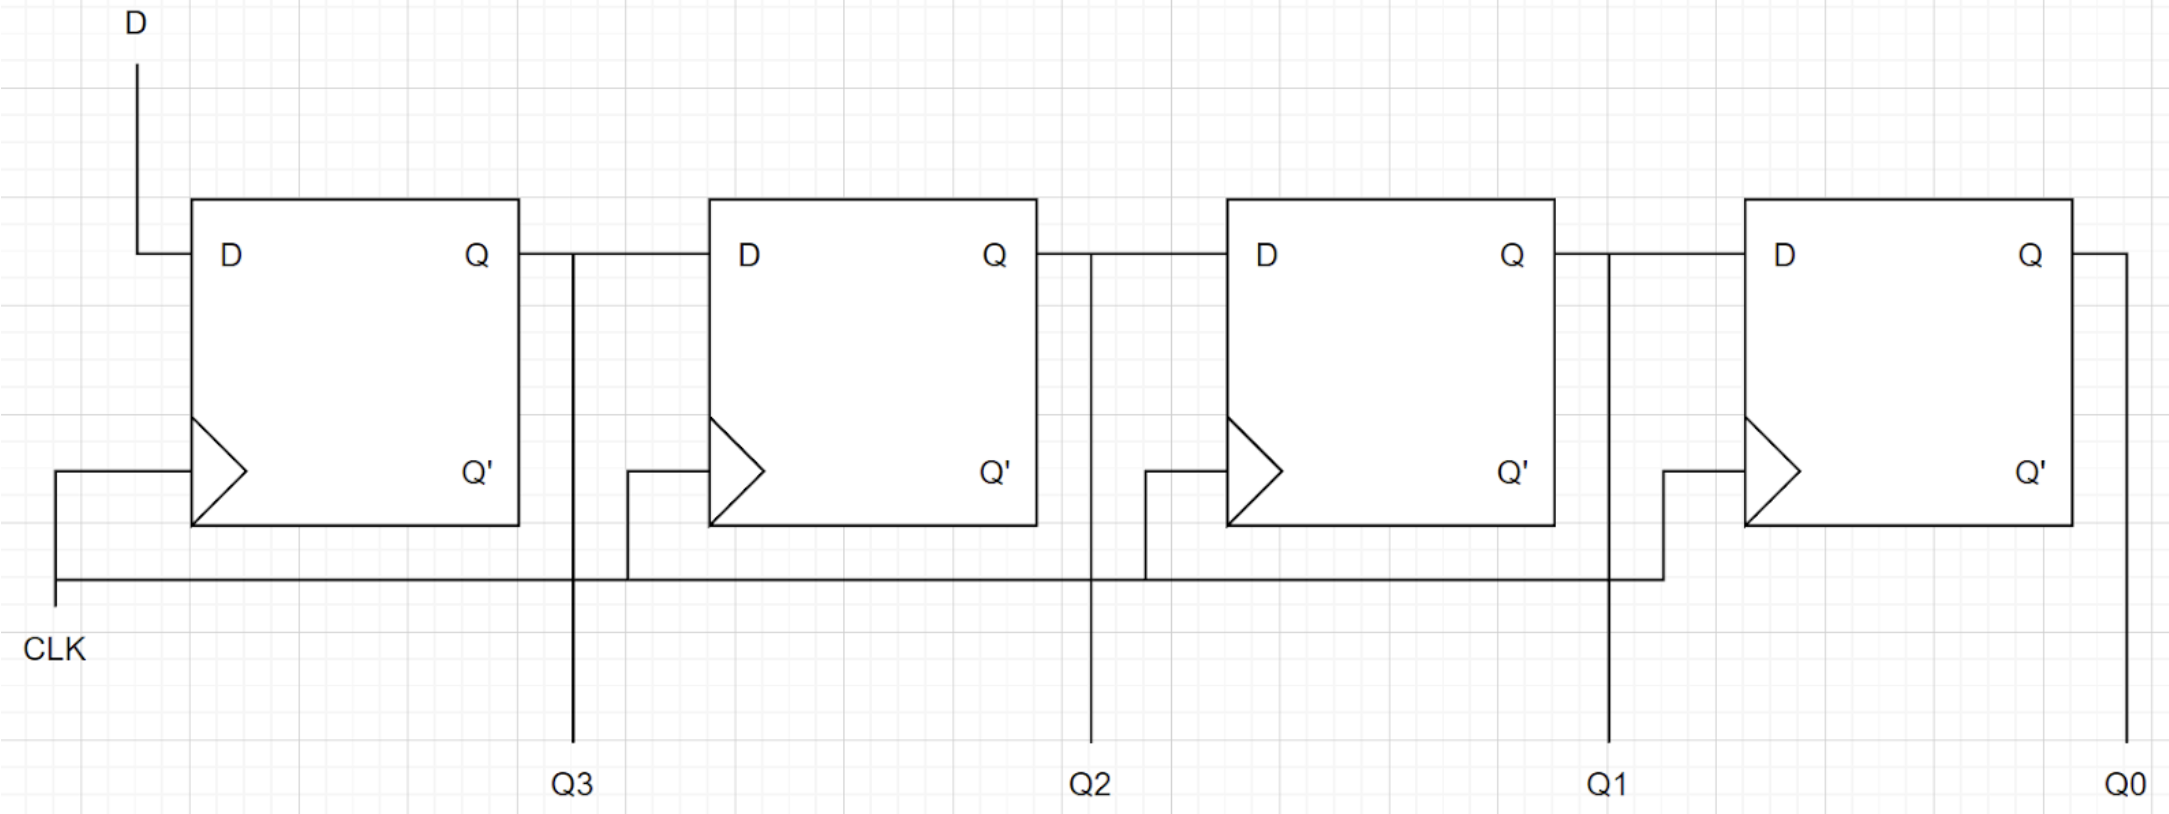
\includegraphics[width=0.9\textwidth]{figures/latch5_solution.png}
\end{figure}


\subsection*{Problem 6}
Implement a 4-bit circular shift register with 4-bit load using D flip-flops.
\begin{figure}[!h]
    \centering
    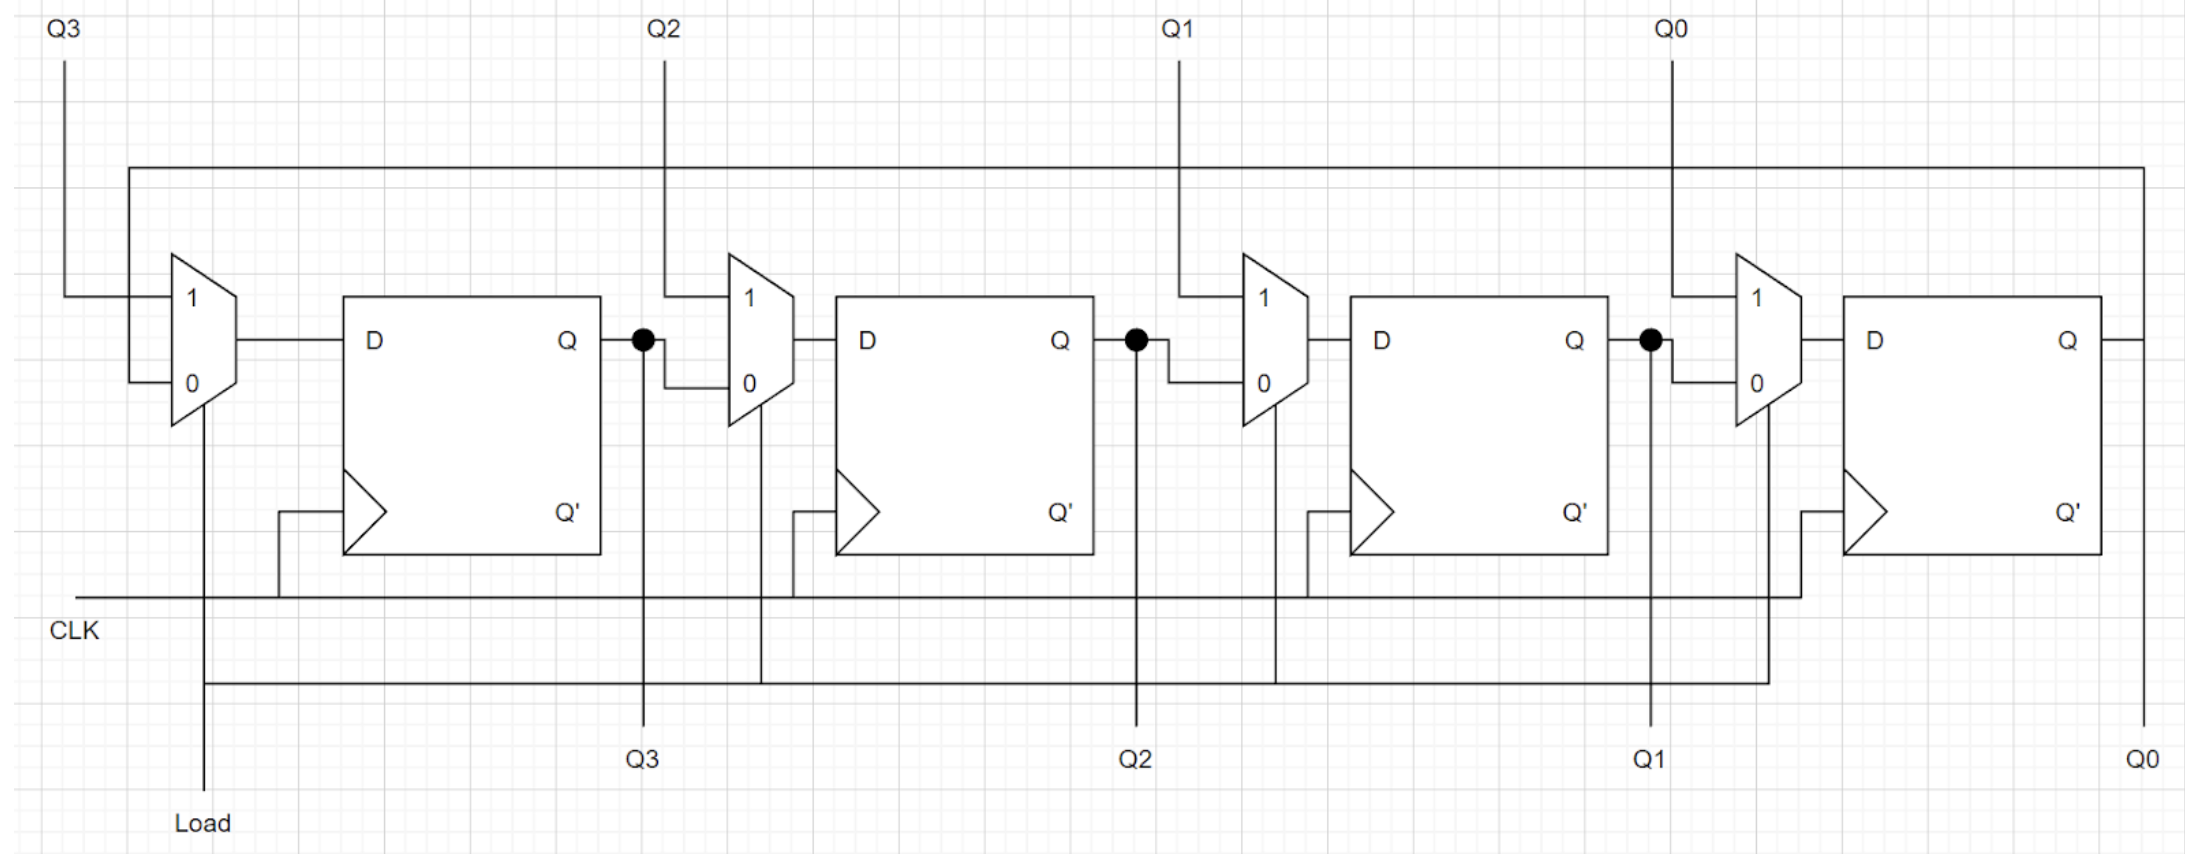
\includegraphics[width=0.9\textwidth]{figures/latch6_solution.png}
\end{figure}

\newpage
\subsection*{Problem 7}
Consider this digital circuit below. \\
\begin{figure}[!h]
    \centering
    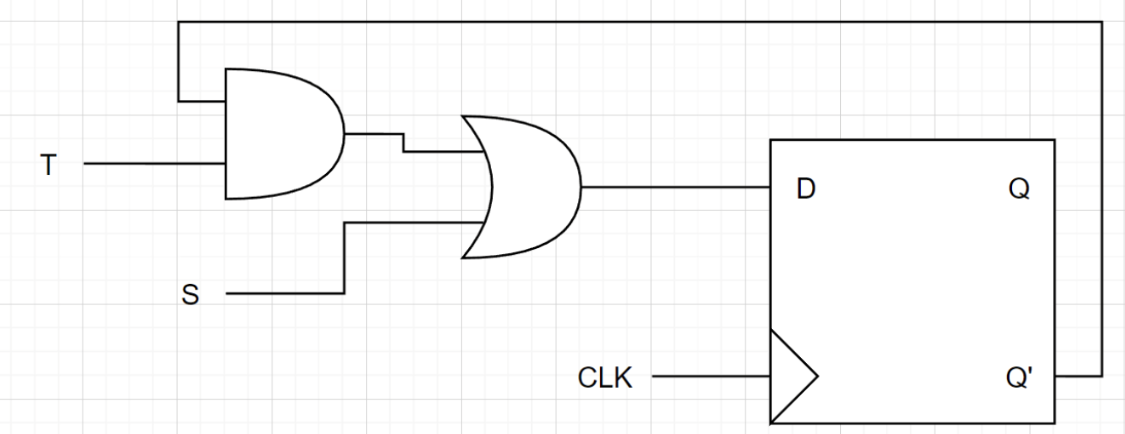
\includegraphics[width=0.7\textwidth]{figures/latch7.png}
\end{figure} \\
Assume at the start, $Q = 0$. Trace and fill out the table below. $T$ and $S$ signals are given in the table.
\begin{table}[!h]
\centering
\begin{tabular}{|l|l|l|l|}
\hline
\textbf{Clock Cycle \#} & \textbf{Q} & \textbf{T} & \textbf{S} \\ \hline
0                       & 0          & 1          & 0          \\ \hline
1                       & 1          & 1          & 0          \\ \hline
2                       & 0          & 0          & 0          \\ \hline
3                       & 0          & 0          & 0          \\ \hline
4                       & 0          & 0          & 1          \\ \hline
\end{tabular}
\end{table}

\subsection*{Problem 8}
What are timing hazards? What are a few ways we can design around them? (Lumetta 2.6.3-2.6.5) \\
\textbf{When we implement a circuit, since gates take time to switch, there may be glitches in our output temporarily (static hazards) or may bounce between outputs until settling to the correct, stable state (dynamic hazards). \\ 
We can design around them by adding additional gates for stability or assign the outputs of unused states to ensure smooth switching.}

\newpage
\section*{Serialized Design}
\subsection*{Problem 1}
Consider one bit-slice of a full adder.
\begin{enumerate}[label=\alph*.]
    \item How many bits need to be passed between each bit slice? What are they? \\
    \textbf{1 bit. We need to pass the carry bit between each bit slice.}
    \item If we wanted to serialize this design and add 1 bit at a time, how many D flip-flops would we need to store these signals? \\
    \textbf{1. We need 1 DFF for each signal we need to store.}
    \item Implement a serialized binary adder, adding 1 bit at a time.
    \begin{figure}[!h]
        \centering
        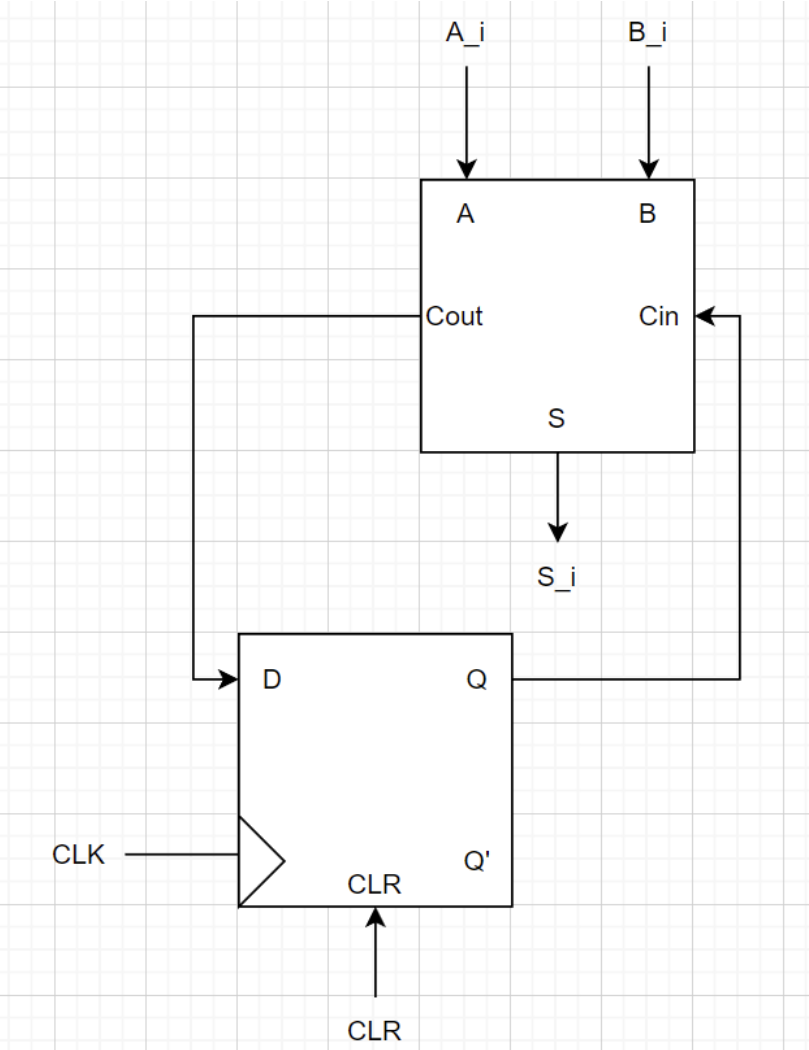
\includegraphics[width=0.6\textwidth]{figures/serial1c_solution.png}
    \end{figure}
    \\ \textbf{Note: the CLR (clear) signal is used when we want to clear the carry bit between adding different sets of numbers.}
    \item Assume we instead wanted to add 4 bits (1 hexadecimal) at a time. Would any signals be different?
    \\ \textbf{No, we still only need to pass one carry bit, the carry bit of the MSB, to the next clock cycle’s LSB.}
    \newpage
    \item Implement a serialized binary adder, adding 4 bits at a time.
    \begin{figure}[!h]
        \centering
        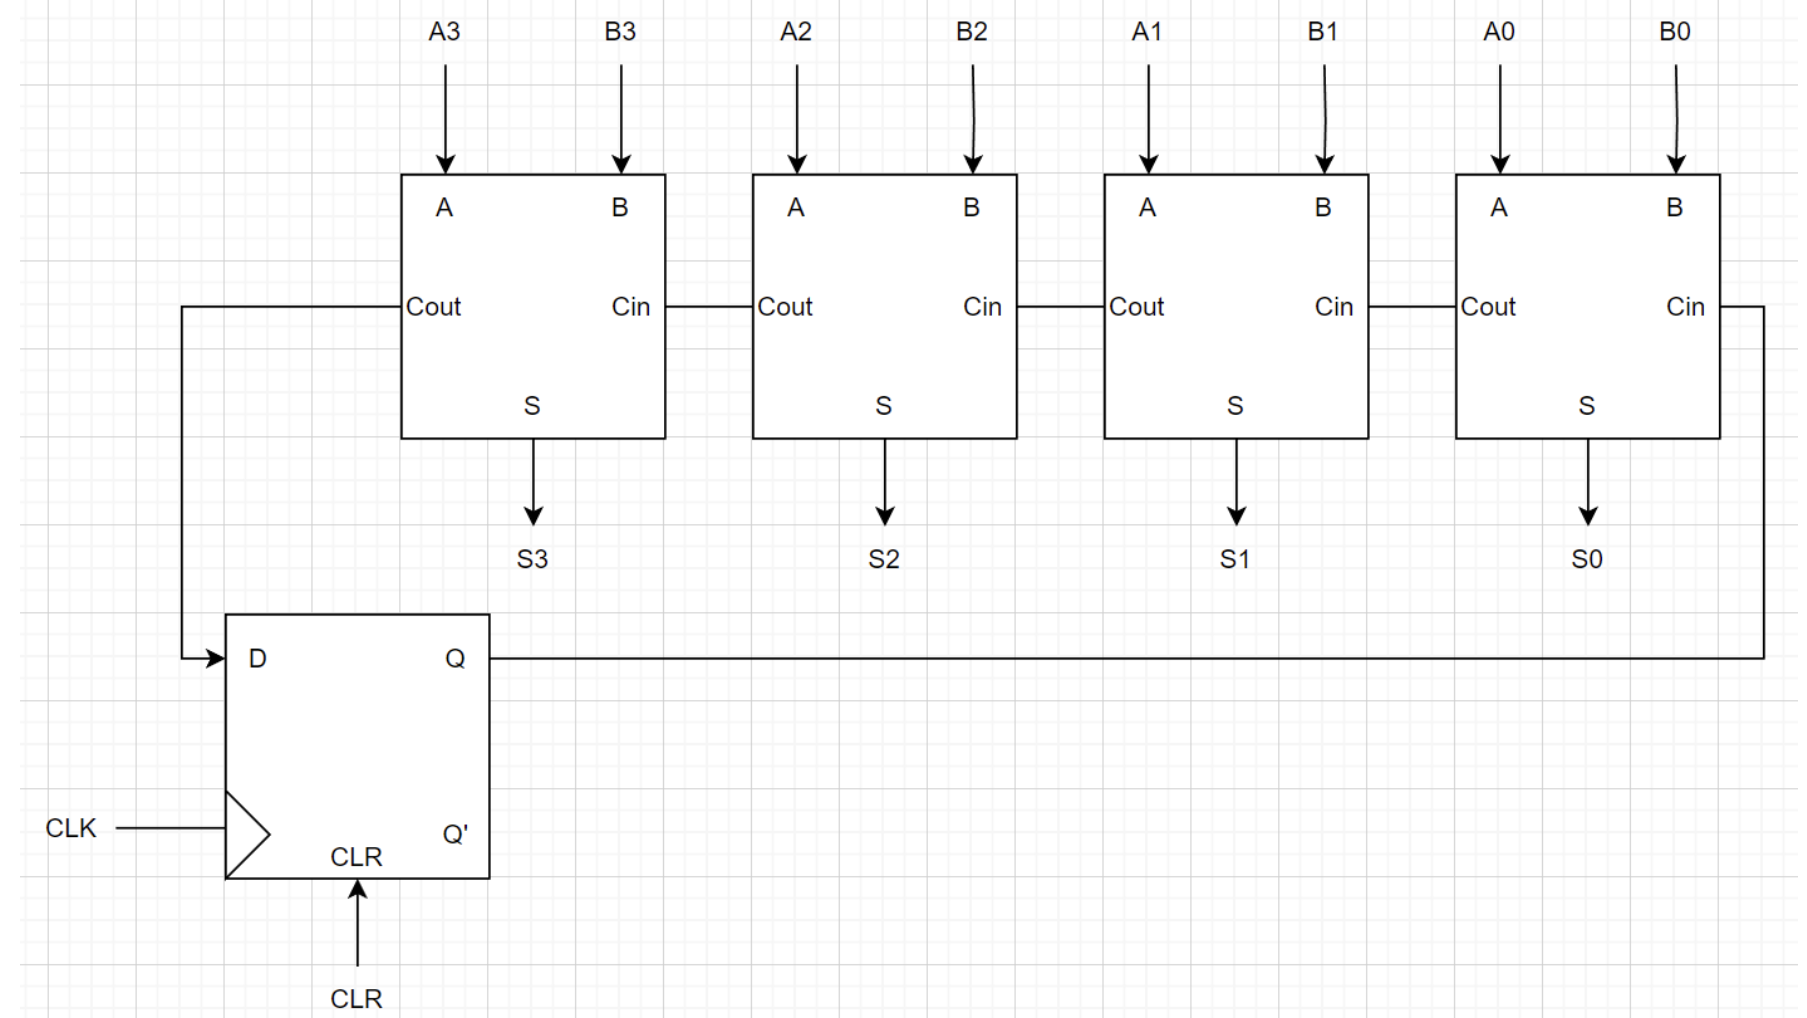
\includegraphics[width=1.1\textwidth]{figures/serial1e_solution.png}
    \end{figure}
\end{enumerate}


\subsection*{Problem 2}
Consider a serialized circuit that takes a sequence of bits, 1 bit at a time, and outputs the same sequence of bits but is delayed by 2 bits and inverted. For example, assuming inputs and outputs are taken at the start of each clock cycle, if the input is 100101101100, then the output is XX0110100100.
\begin{enumerate}[label=\alph*.]
    \item How many bits do we need to store between each clock cycle? \\
    \textbf{2 bits.}
    \item Implement this circuit using D flip-flops.
    \begin{figure}[!h]
        \centering
        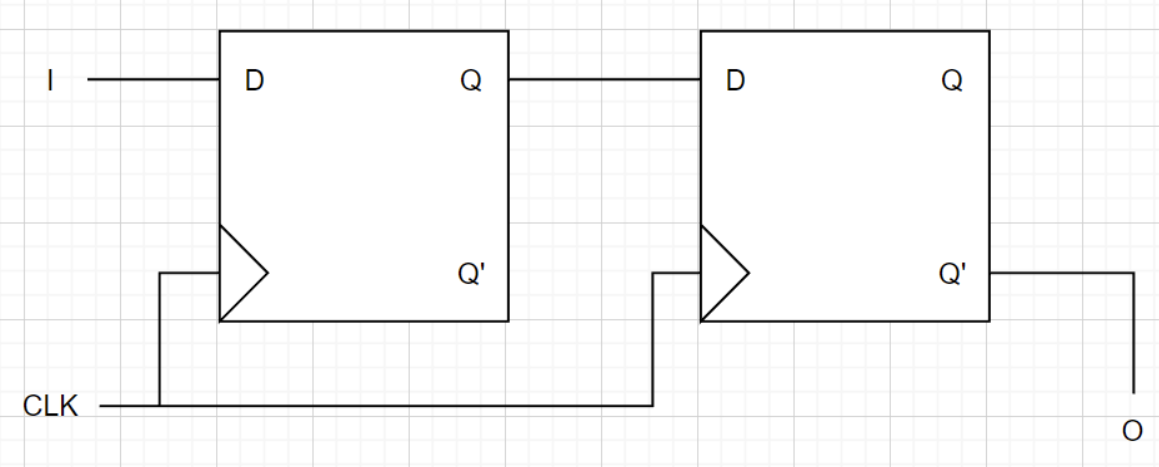
\includegraphics[width=1\textwidth]{figures/serial2b_solution.png}
    \end{figure}
    \item Can we also implement this circuit using a shift register? \\
    \textbf{Yes:}
    \begin{figure}[!h]
        \centering
        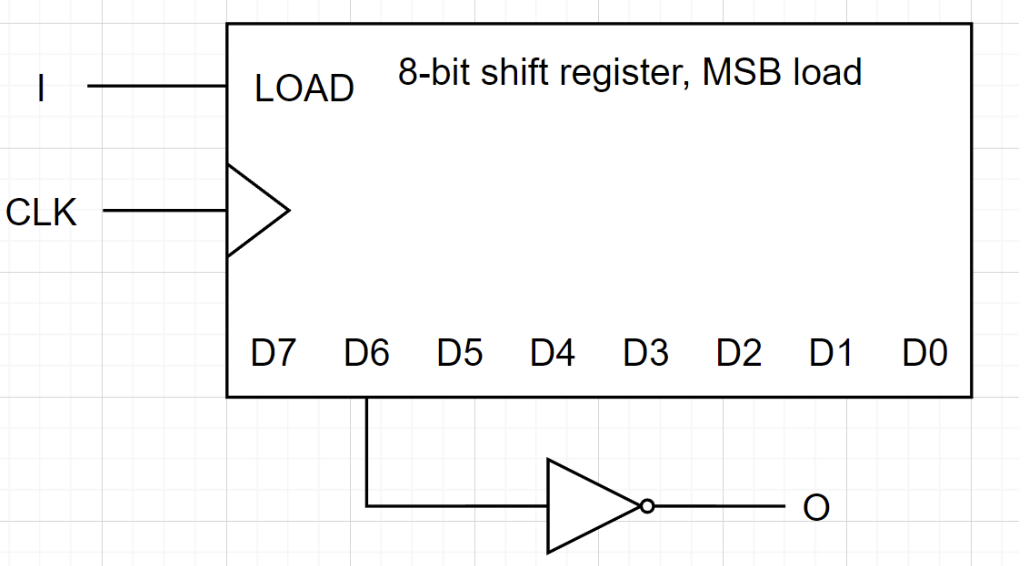
\includegraphics[width=0.8\textwidth]{figures/serial2c_solution.png}
    \end{figure}
\end{enumerate}


\subsection*{Problem 3}
In 50 words or less, what are the advantages and disadvantages of serialization over bit-slicing?\\ 
\\ \textbf{For larger sequences, serialized designs take much less area than bit-sliced designs. However, serialized designs are much slower, as they depend on the speed of a clock signal, while bit-sliced design is only dependent on gate delay. }

\end{document}